%\PassOptionsToPackage{unicode=true}{hyperref} % options for packages loaded elsewhere
%\PassOptionsToPackage{hyphens}{url}
%
\documentclass[a4paper,14pt,openany,final]{extreport} % с экрана надпись надо убрать
%\usepackage[times,fancytop,firamono,cpcaption,microtyping]{subook}
\usepackage[times,firamono,microtyping,irnitu,732,asanamath,tinytitles]{subook} % 732,asanamath
%\usepackage{booktabs}
\usepackage{multicol}
\usepackage{totcount}
\usepackage{multirow}
\usepackage{array}
\usepackage{makecell}
\usepackage{titlesec}
\usepackage{enumitem}
\usepackage{newfloat}
\usepackage{caption}
% \usepackage{tocloft}
\graphicspath{{./pics/}}
\renewcommand{\chaptername}{}
\makeatletter
\makeatother

%\usepackage{color}
%\usepackage{soul}
\date{}
% \hypersetup{
%     bookmarks=true,         % show bookmarks bar?
%     unicode=true,           % non-Latin characters in Acrobat’s bookmarks
%     pdftoolbar=true,        % show Acrobat’s toolbar?
%     pdfmenubar=true,        % show Acrobat’s menu?
%     pdffitwindow=false,     % window fit to page when opened
%     pdfstartview={FitH},    % fits the width of the page to the window
%     pdftitle={Компьютерные науки, часть 4},    % title
%     pdfauthor={Евгений Александрович Черкашин},     % author
%     pdfsubject={Методическое пособие},   % subject of the document
%     pdfcreator={EMACS-24.4:AuCTeX},   % creator of the document
%     pdfproducer={LuaLaTeX}, % producer of the document
%     pdfkeywords={Искусственный интеллект} {Логическое
%       программирование} {Планирование действий} {Удовлетворение
%       ограничений} {Компьютерная алгебра} {Принцип максимума} {Оптимальное управление}, % list of keywords
%     pdfnewwindow=true,      % links in new window
%     colorlinks=true,       % false: boxed links; true: colored links
%     linkcolor=[rgb]{0 0.4 0.1},          % color of internal links (black)
%     citecolor=blue,        % color of links to bibliography
%     filecolor=black,      % color of file links
%     urlcolor=[rgb]{0.3 0.0 0.3}           % color of external links
%   }

% \let\oldcaption\caption
%\renewcommand{\caption}[1]{\stepcounter{lastfig}\label{LastFig}\oldcaption{#1}}

\newcommand\theyear{2018}

\usepackage{xcolor}
\usepackage{stackengine}
\setstackgap{L}{.5\baselineskip}
\newcommand\MA[2]{{\sffamily\color{red}\hsmash{$\uparrow$}%
  \smash{\toplap{#1}{\scriptsize\bfseries #2}}}}
\newcommand\MB[2]{{\sffamily\color{red}\hsmash{$\downarrow$}%
    \smash{\bottomlap{#1}{\scriptsize\bfseries#2}}}}
\usepackage{tikz}

\newcommand*{\hl}[1]{%
\tikz[baseline]\node[rectangle, fill=yellow, rounded corners, inner sep=0.3mm,anchor=base]{#1};%
}
\makeatletter
   \def\vhrulefill#1{\leavevmode\leaders\hrule\@height#1\hfill \kern\z@}
\makeatother

\newcommand\toprule{\noindent\vhrulefill{2pt}}
\newcommand\bottomrule{\noindent\vhrulefill{2pt}}
\newcommand\midrule{\noindent\vhrulefill{2pt}}

\newtotcounter{captionsnum}
\def\oldcaption{} \let\oldcaption=\caption
\def\caption{\stepcounter{captionsnum}\oldcaption}

\newtotcounter{bibitemnum}
\def\oldbibitem{} \let\oldbibitem=\bibitem
\def\bibitem{\stepcounter{bibitemnum}\oldbibitem}

\newtotcounter{appsnum}
\setcounter{appsnum}{1}

\newcommand\T{\rule{0pt}{2.6ex}}       % Top strut
\newcommand\B{\rule[-1.2ex]{0pt}{0pt}} % Bottom strut
\newcommand{\BA}[1]{%
  \begin{minipage}[b]{0.4\textwidth}
    \raggedright\T
    #1
  \end{minipage}
}
\let\BT\BA
\newcommand{\BB}[1]{%
  \begin{minipage}[t]{0.4\textwidth}
    \raggedright\T
    #1
  \end{minipage}
}
\newcommand{\BC}[2]{%
  \begin{minipage}[c]{#1}
    \raggedright\T
    #2
  \end{minipage}
}

% Убрать марки и выделения.
\providecommand\hl[1]{}
\renewcommand\hl[1]{#1}
\renewcommand\MA[2]{}
\renewcommand\MB[2]{}
\renewcommand{\bibname}{Список использованных источников}
\providecommand\sfcpshape{\rmfamily}
\newcommand{\capfont}{\Large\sffamily\sfcpshape\bfseries}
\usepackage{pifont}

% setup list parameters
\setlist{itemsep=0pt plus 0.1pt,topsep=0pt plus 0.3pt,parsep=0pt plus 0.7pt}
\setlist[itemize]{label=\ding{113}}


\DeclareFloatingEnvironment[fileext=pzlst,placement={!hbtp},name=Листинг]{pzlisting}
\captionsetup[pzlisting]{format=hang,labelsep=ddash,singlelinecheck=on,font={small},labelfont={small},textfont={small},labelfont={normalfont},justification=justified,skip=0.2ex}

% \setcitestyle{numbers,square}
\usepackage{minted} % пора заканчивать. завтра в 7 у меня другая срочная работа. Половина текста сделана.
%\setmainfont{Brill} % Для разнообразия. Таймс задолбал.
%\addfontfeature{Numbers=Lining}
\begin{document}
\renewcommand{\bibname}{СПИСОК ИСПОЛЬЗОВАННЫХ ИСТОЧНИКОВ}
\renewcommand{\chaptername}{}
\clubpenalty=10000
\widowpenalty=10000
\parskip=0pt plus 1pt

\tableofcontents

\chapter*{ВВЕДЕНИЕ}

Каждый человек рано или поздно сталкивается с проблемой выбора на рынке недвижимости.  Принимаемые в это время решения значительно влияют на дальнейшую жизнь семьи, организации, фирмы и т.д.
Поэтому всякая помощь на этом этапе представляется необходимым моментом.  Для поддержи принятия решения существует целая индустрия -- услуги риелторов, задач которых организовывать процесс поиска интересующих объектов недвижимости на рынке, обеспечение безопасности сделки, соответствующий документооборот.

С другой стороны, на рынке недвижимости Иркутской области находятся много различных уникальных объектов, которые уже долгое время не могут найти себе рачительного хозяина, способного эффективно эту собственность ввести в эксплуатацию.  Как следствие, продавцы терпят убытки, платя налоги за нерентабельную собственность, а у покупателей нет возможности инвестировать свободные капиталы.  Причина такой ситуации -- неразвитость информационного обеспечения, т.е. несмотря на активную рекламу таких объектов риелторским конторам не удается найти покупателя.

Деятельность риелторов в некоторой степени автоматизируется.  Офисные пакеты используются для подготовки документации, ведется бухгалтерия, а также существуют сетевое программное обеспечение, которое организует и регламентирует взаимоотношения риелторов друг с другом, и с сервисами услуг оценки объектов и рынка недвижимости в целом.  При помощи таких CRM организуются сделки между риелторами: на некоторую плату объект передается другому риелтору на продажу, -- контроль ранних договоренностей.

С другой стороны, согласно рекламе сайта Avito, каждая вторая квартира продается именно через интернет--сайты без участия риелторов.  Опрос риелторов показал, что это не совсем так.  Многое зависит от <<традиций>> того или иного региона Российской Федерации.  Например, в Иркутской области и Москве недвижимость предпочитают продавать через интернет"=сайты, причем делается несколько предложений одной и той же квартиры на нескольких сайтах.  Опыт показывает, что это практически всегда приводит к тому, что цена на объект недвижимости падает ниже рыночной.  В Екатеринбурге, наоборот, недвижимость преимущественно продается через риелторские конторы, что и стабилизирует цены на жилье, и делает процесс купли"=продажи более предсказуемым для продавца.

В таблице \ref{tab:market-irk} представлены количественные характеристики роста рынка недвижимости Иркутской области.. В период с 2010 по 2016 год количество сделок только по жилой недвижимости на вторичном рынке выросло примерно на 20\%. Ежегодно в Иркутской области вводится в эксплуатацию не менее 30~000 новых квартир.
На сайте Avito.ru выставлены на продажу более 5~000 квартир, находящихся на территории Иркутской области.

\begin{table}[htb]
  \caption{Характеристика рынка недвижимости Иркутской области}
  \label{tab:market-irk}
  \centering
  \begin{tabular}{|c|c|}
    \hline
Год &
      Количество сделок \\
    \hline
2010 &
12594 \\
2011 &
13756 \\
2012 &
15080\\
2013 &
14540\\
2014 &
15651\\
2015 &
15005\\
2016 &
       15982\\
    \hline
\end{tabular}
\end{table}

Таким образом, для гармонизации процессов на рынке недвижимости имеет смысл разработать информационную систему, которая не только бы сообщала актуальную информацию об объектах недвижимости, но и помогала бы искать такие объекты покупателям.  Такой сервис должен функционировать на основе современных методов анализа и структуризации данных: выбирать для конкретных пользователей объекты недвижимости, которые потенциально могил бы его заинтересовать.  Такими системами в разных предметных областях выступают \emph{рекомендательные системы} (РС).

Рекомендательные системы \cite{b1} -- информационные систем поддержки принятия решений, предназначенные для оценки уровня интереса пользователя к определенному продукту или сервису объекту на основе имеющейся информации о пользователе и/или объекте. Отрасль разработки РС начала активно развиваться при появлении онлайн"=сервисов продаж, и в настоящее время РС – одно из активных направлений развития систем поддержки принятия решений, ориентированное, прежде всего, на коммерческое использование, а также на решение задач повышения продуктивности поиска релевантной информации.

В коммерции РС позволяют решать задачи установления, что именно представляет ценность для потребителя в виде набора конкретных объектов (например, товаров или услуг), сужение вариантов выбора и предоставление схожих вариантов других объектов, тем самым упрощая выбор. РС позволяют также выявлять новые характеристики объектов, например, при помощи ведения классификаций объектов и анализа набора известных признаков. Использование РС позволяет отделам снабжения коммерческих фирм-поставщиков предоставлять уникальный сервис каждому потребителю, увеличивая его доверие и лояльность к поставщику, увеличивая продажи и конверсию, а также получая и накапливая больше знаний о потребителях.

Рекомендательные системы появились в интернете достаточно давно, около 20 лет назад. Однако настоящий подъем в этой области случился примерно 5-10 лет назад, когда произошло соревнование Netflix Prize. Компания Netflix тогда давала в прокат не цифровые копии, а рассылала VHS-кассеты и DVD. Для них было очень важно повысить качество рекомендаций. Чем лучше Netflix рекомендует своим пользователям фильмы, тем больше фильмов они берут в прокат. Соответственно, растет и прибыль компании. В 2006 году они запустили соревнование Netflix Prize. Они выложили в открытый доступ собранные данные: около 100 миллионов оценок по пятибалльной шкале с указанием ID проставивших их пользователей. Участники соревнования должны были как можно лучше предугадывать, какую оценку поставит определенному фильму тот или иной пользователь. Качество предсказания измерялось при помощи метрики RMSE (средне-квадратичное отклонение). У Netflix уже был алгоритм, который предсказывал оценки пользователей с качеством 0.9514 по метрике RMSE (см.~раздел~\ref{sec:rs-eval}). Задача была улучшить предсказание хотя бы на 10\% — до 0.8563. Победителю был обещан приз в \$1~000~000. Соревнование длилось примерно три года. За первый год качество улучшили на 7\%, дальше все немного замедлилось. Но в конце две команды с разницей в 20 минут прислали свои решения, каждое из которых проходило порог в 10\%, качество у них было одинаковое с точностью до четвертого знака. В задаче, над которой множество команд билось три года, все решили каких-то двадцать минут. Опоздавшая команда (как и многие другие, участвовавшие в конкурсе) остались ни с чем, однако сам конкурс очень сильно подстегнул развитие в этой области [2].

% TODO: Цели, задачи, требования

\paragraph{Целью}\hspace{-1em} данной выпускной квалификационной работы магистранта является проектирование и реализация рекомендательной системы для рынка недвижимости Иркутской области, применимой для решения перечисленных выше проблем.

Для достижения цели \textbf{решены следующие задачи}:
\begin{enumerate}
\item Анализ предметной области рекомендательных систем и рынка недвижимости;
\item Тестирование разработанной рекомендательной системы.
\end{enumerate}

К создаваемому программному обеспечению выдвигались следующие дополнительные \textbf{требования}:
\begin{enumerate}
\item система должна вырабатывать рекомендации в режиме <<холодного старта>>;
\item не принуждать пользователей к регистрации и авторизации, но при этом обеспечивать накопление необходимой информации;
\item тестирование системы должно производится на данных рынка недвижимости Иркутской области, что обеспечивает экспертную оценку рекомендаций;
\item программное обеспечение необходимо реализовать преимущественно на свободных (\foreignlanguage{english}{open-source)}) технологиях.
\end{enumerate}

\chapter{ТЕХНОЛОГИИ РАЗРАБОТКИ ИНФОРМАЦИОННЫХ ИНТЕРНЕТ"=СИСТЕМ}
\label{chap:dev-tech-theory}

В данном разделе рассматриваются технологии, которые использованы для проектирования и реализации рекомендательной системы для рынка недвижимости Иркутской области.

\section{Рекомендательные системы}
\label{sec:domain-descr}

В области рекомендательных систем используется специальная терминология. \emph{Объектом} обозначается то, что система рекомендует \emph{пользователям}, например, продукты, услуги, товары, новости, книги, DVD и т.п. \emph{Профилем пользователя} или \emph{объекта} являются данные, характеризующие пользователя или объект. Именно эти данные используются в процессе оценивания \emph{релевантности} объекта к желаниям пользователя. Этот процесс называется \emph{фильтрацией} (\foreignlanguage{english}{filtering}). В результате фильтрации объекты \emph{ранжируются} в соответствии с полученной оценкой, а пользователю предоставляется некоторое конечное подмножество, элементы которого имеют максимальную релевантность, т.е. оцениваются как наиболее интересные пользователю. Далее под \emph{интересом} будем понимать именно интерес пользователя к объекту. Т.к. РС -- это, прежде всего, информационные системы, то все объекты и пользователи описываются при помощи \emph{атрибутов}. Именно атрибуты являются входной информацией во все процедуры оценивания интереса. \emph{Качество рекомендации} -- оценка точности предсказания интереса, сделанного РС, например, в сравнении с имеющимися примерами, т.е. оценками конкретных объектов конкретными пользователями.

Рекомендательные системы полезны не только для информационных ресурсов и порталов электронной коммерции, но и могут также открыть новые возможности в области безопасности, автомобильной промышленности [3], рекламе [4] и др.
Существует ряд подходов к оценке интереса.

Существует ряд подходов к оценке интереса:
\begin{enumerate}
\item на основе \emph{фильтрации содержания}
  (\foreignlanguage{english}{content-based information filtering}), при этом в информационной
  системе создаются профили пользователей и объектов, включающие
  социальный статус пользователя, возраст, место проживания, род
  деятельности, а также характеристики, выражающие интерес
  пользователя к объекту; профили объектов включают позицию в системе
  классификации, его потребительские характеристики. % вакханалия
\item	на основе\emph{ коллаборативной фильтрации} (\foreignlanguage{english}{collaborative filtering}), где используется информация о поведении пользователей в прошлом, например, перечень покупок или оценок объектов, сделанных на сайте интернет-магазина в прошлом пользователями из той же группы интересов, при этом аналитическим блоком информационной системы автоматически формируются классификации объектов, производится \emph{ранжирование атрибутов} по степени значимости в оценке интереса.
\item	\emph{интеллектные} (knowledge-based), где оценка вычисляется на основе формализованных знаний.
\item	\emph{гибридные} (\foreignlanguage{english}{hybridprediction}) методы, которые базируются на подходах пп. 1 и 2, включая элементы из 3, что призвано повышать эффективность 1 и/или 2.
\end{enumerate}

Например, в Music Genome Project музыкальный аналитик оценивает каждую композицию по сотням различных музыкальных характеристик, при помощи которых выявляются музыкальные предпочтения пользователя. Перечень оценок формирует \emph{профиль музыкального произведения}. Основная проблема первого типа РС (фильтрации содержания) — это работоспособность системы на начальном этапе ее эксплуатации, так называемый <<\emph{холодный старт}>>: для новых пользователей в системе нет необходимой информации в профиле для принятия решения о том, какие объекты следует предлагать. В связи с этим в современных рекомендательных системах реализуется механизм сбора и анализа данных о пользователях с применением \emph{явных} и \emph{неявных методов}.

Явные методы сбора данных выполняют следующие действия:
\begin{itemize}
\item запрос у пользователя оценки объекта по некоторой шкале;
\item запрос у пользователя ранжировки группы объектов от наилучшего к наихудшему;
\item предъявление пользователю двух объектов с вопросом о том, какой из них лучше;
\item предложение создать список объектов, характеризующих предпочтения пользователя.
\end{itemize}
Примерами неявного сбора данных выступают:

\begin{itemize}
\item наблюдение за тем, что просматривает пользователь в
  интернет-магазине или базе данных;
\item ведение записей о поведении
  пользователя онлайн.
\end{itemize}
Сбор информации из социальных сетей, например, как в [5-7].

Второй тип РС, основанные на коллаборативной фильтрации, сравнивают однотипные данные, полученные от разных людей и вычисляют список рекомендаций для конкретного пользователя. Для вычисления рекомендаций используется, например, граф интересов. Таким образом, РС представляют собой информационные системы, дополненные алгоритмами, позволяющими обнаружить в хранилище объекты, которые не имеют непосредственного отношения к запросу пользователя. Любопытно, что рекомендательные системы часто используют как поисковые машины для индексации необычных данных.

Более подробное описание различных подходов к реализации подсистем РС рассмотрим на примерах из современной литературы.

\section{Примеры использования РС}
\label{sec:rs-examples}

В обзоре \cite{b8} рассмотрены РС в области предоставления пользователям текстовых документов, в частности, научных статей. Больше половины (55\%, 34 из 62) систем построены на основе фильтрации содержания. Алгоритмы коллаборативной фильтрации использованы только в 18\% (11 из 62) случаев. Представлены подходы, основывающиеся на стереотипировании и гибридных методах. Авторы исследования пришли к выводу, что в 81\% случаев моделирование пользователя на основе автоматического сбора информации не приносит значимых результатов по сравнению с явным указанием набора ключевых слов.

В основе характеристик объектов, научных статей, в исследованных РС используют просто ключевые слова, содержащиеся в документах, реже \(N\)-граммы, а также нетекстовые элементы, такие как ссылки на другие статьи и фамилии авторов. Самая популярная модель для хранения представления статей -- модель векторного пространства. Моделирование пользователя осуществляется при помощи графов и списков тем, назначенных пользователям в результате машинного обучения. Темы объединяются в иерархические справочники, например, на основе классификаторов АСМ. В рассмотренных подходах тексты извлекаются из заглавий, аннотаций, заголовков, введения, предисловия, предоставленных автором ключевых слов, библиографии, основного текста, социальных тегов и цитирований контекста.

В РС, где применялась коллаборативная фильтрация, и ни в одном из проектов не удалось успешно использовать явные рейтинги: пользователи были слишком ленивы, чтобы самостоятельно задавать рейтинг статьям. Неявные рейтинги получены из данных по количеству страниц, прочитанных пользователем, взаимодействию пользователей с документами (загрузка, редактирование, представление) и цитирования. Главная проблема коллаборативной фильтрации для научных работ -- это дефицит информации, например, для РС научных статей Mendeley по сравнению с Netflix (онлайн фильмы) дефицит составляет три порядка.  Неявные рейтинги объектов получаются из анализа одновременной загрузки статьи (со"=загрузка) разными пользователями одной группы, совместного просмотра (со"=просмотр), совместное цитирование статьями (со"=цитирование) одних и тех же источников. Оказалось, что со"=цитирование, будучи эффективным в начале появления статьи на сервисе РС, через два года начинает уступать со"=загрузке. Популярным подходом представления результата такого анализа являются графы. Вершины графа -- это статьи, представленные наборами атрибутов, а дуги -- соотношения между статьями.

Основными проблемами в области РС являются следующие:
\begin{itemize}
\item отсутствие общего базиса оценивания качества систем (по
  предметным областям), включая объективную информацию о реальных
  оценках реальных пользователей, нестабильность методов оценивания и
  высокая их зависимость от <<шума>>;
\item неиспользованный потенциал
  научных исследований: новые научные результаты не внедряются в
  практические приложения (большинство работающих РС базируются на
  простых методах), данные существующих практических реализаций РС
  научно не исследуются, нет тесного взаимодействия со снежными
  областями анализа данных, а так же друг с другом, низкий научный
  интерес к РС;
\item в оценке удовлетворенности не учитывается факторы
  конфиденциальность, безопасности данных, разнообразие, разметка и
  презентация информации; в значимом количестве РС моделирование
  пользователя было крайне примитивно - набор ключевых слов,
  собственная статья или просто фрагмент текста, представляющих
  научные интересы пользователя.
\end{itemize}
    Среди открытых проектов выделяются MyMediaLite, LensKit, Mahout, Duine, RecLabCore, Easyrec и Recommender.

\subsection{Методы фильтрации содержания}
\label{sec:content-filtering}

В статье \cite{b5} решается задача анализа профиля пользователя в социальной сети ВКонтакте для решения проблемы холодного старта в решении задачи рекомендации жанров и произведений музыки и фильмов. Авторами разработана РС «EZSurf» автоматизирующая процесс веб"=сёрфинга и фильтрации контента, используя профиль пользователя в социальной сети <<ВКонтакте>>, а также API сервисов last.fm, TheMovieDB для получения сведений о схожих объектах (музыкальных произведений). Такой подход существенно упрощает хранилище данных РС, поскольку не требует создания собственной системы классификаций и базы объектов.

В статье \cite{b9} рассматривается задача выделения $N$ объектов с наивысшими оценками интереса, задача top"=$N$, при применении фильтрации контента. Предлагается математическая модель контентной рекомендательной системы, основанная на нечетких множествах, критерий оценки качества рекомендаций и алгоритм решения задачи. Математическая модель и алгоритм протестированы на данных сайта last.fm.

\subsection{Методы коллаборативной фильтрации}
\label{sec:collab-filtering}

Подходы, основанный на коллаборативной фильтрации, в настоящее время более популярны, чем подходы на основе фильтрации содержимого, вероятно из-за того, что представляет собой отражение практического опыта: большинство коммерческих РС вынуждены решать проблему недостатка информации, <<холодный старт>>, а также адаптируемости существующих сообществ пользователей к новым объектам.

Суть идеи коллаборативной фильтрации изображена на рисунке~\ref{fig:collab-essence}. Пользователям предоставляются интересующие их товары, которые они оценивают «положительно» или «отрицательно» пока пользуются сайтом, например, интернет"=магазином.

\begin{figure}[htb]\centering
  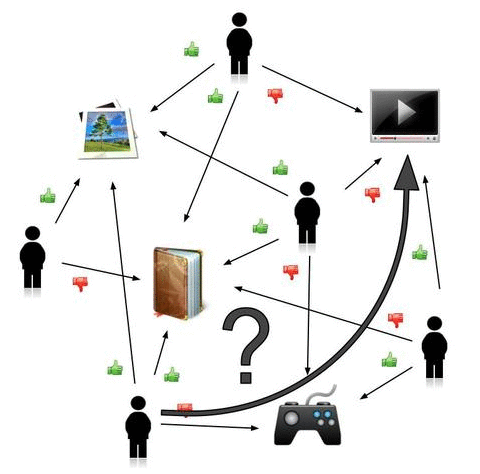
\includegraphics[width=0.5\linewidth]{collab1.png}
\caption{Накопление рейтингов покупателей о товарах}
\label{fig:collab-essence}
\end{figure}

Накопленные данные записывается в таблицу, которая представлена на рисунке~\ref{fig:collab2}, где столбцы -- это объекты, т.е. товары, а строки -- это оценки пользователей.
\begin{figure}[htb]
  \centering
  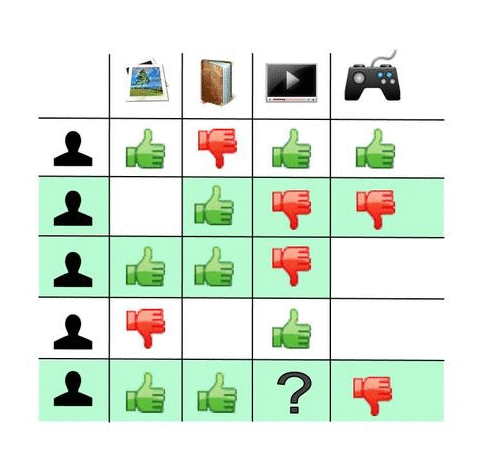
\includegraphics[width=0.5\linewidth]{collab2.png}
  \caption{Таблица собранной информации об оценках товаров пользователями}
  \label{fig:collab2}
\end{figure}

Задача рекомендательной системы, заключается в заполнение <<всех>> ячеек, помеченных вопросительным знаком на рисунке~\ref{fig:collab2}.

Для оценки интереса пользователя к объекту, помеченному вопросительным знаком, сравниваем пятого (последнего) пользователя со всеми остальными пользователями по критерию схожести его выбора. Пользователи под номерами «пять» и «три», схожи по первым двум товарам, т.к. оба ответили «положительно» по данным товарам. Пользователи под номерами «пять» и «два», схожи по товарам под номерами «два» и «четыре», т.к. оба ответили одинаково «положительно» на товар под номером «два» и «отрицательно» под номером «четыре». Следовательно, можно предположить, что пользователь под пятым номером скорее всего отнесется «отрицательно» к товару под номером «три», что представлено на рисунке~\ref{fig:collab3}.

\begin{figure}[htb]
  \centering
  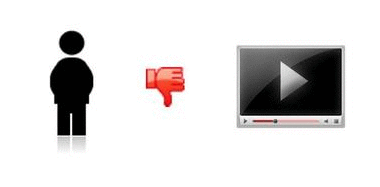
\includegraphics[width=0.5\linewidth]{collab3.png}
  \caption{Пример рекомендации}
  \label{fig:collab3}
\end{figure}

	Полученная оценка означает, что пользователю данный товар будет показываться в последнюю очередь.


Математические обозначения элементов модели сравнения состоит из набора пользователей $U$  и набора объектов $O$. Тогда $O_u$ -- это множество элементов, оцененных пользователем $u$, $U_0$ -- множество пользователей, которые оценили объект $o$, $r_{u,o}$ -- оценка пользователя $u$ для объекта $o$, $\mathbf{r}_u$ -- вектор всех оценок пользователя $u$, $\mathbf{r}_o$  -- вектор всех оценок объекта $o$, $\bar{r}_u$ и $\bar{r}_o$ -- средние значения оценок пользователя $u$ и объекта $o$,   соответственно. Сравнительная оценка обозначается $\hat{r}_{u,i}$. Для задания этой оценки сначала задается мера близости объекта $i$ к объекту $j$. Рассмотрим несколько популярных вариантов оценки близости.

Коэффициент Пирсона [3]:
\[
  s_{i,j}=\frac{\sum\limits_{u\in U}(r_{u,j}-\bar{r}_i)(r_{u,j}-\bar{r}_j)}{\sqrt{\sum\limits_{u\in U}(r_{u,j}-\bar{r}_i)^2}\sqrt{\sum\limits_{u\in U}(r_{u,j}-\bar{r}_j)^2}}
\]
где $U=U_i\cup U_j$ -- множество пользователей, которые оценили объекты $i$ и $j$.

Косинус угла между двумя векторами $\mathbf{r}_i$ и $\mathbf{r}_j$:
\[
  s_{i,j}=\cos(\mathbf{r}_i,\mathbf{r}_j)=\frac{\mathbf{r}_i \cdot \mathbf{r}_j}{|\mathbf{r}_i||\mathbf{r}_j|}.
\]
Затем производится формирование конечного множества объектов $S$ наиболее близких к объекту $o$. Вычисление рейтинга объекта $o$ делается по формуле:
\[
  \hat{r}_{u,o}=\frac{\sum\limits_{j\in S}S_{o,j}\cdot r_{u,j}}{\sum\limits_{j\in S}|S_{o,j}|}.
\]

Популярный подход к формированиюмножества рекомендаций -- это упорядочивавшие всех объектов по критерию схожести и выборке некоторого фиксированного количества объектов с максимальным рейтингом [Нефедова]. В качестве меры схожести (\foreignlanguage{english}{similarity}) двух объектов выступает $\cos$ угла между $N$-мерными векторами.

В [3,10] так же представлен обзор способов использования вышеупомянутых методов вычисления оценок, которые разделены на два класса -- \emph{анамнестические}, т.е. основывающиеся на одновременной обработке всех имеющихся данных, и \emph{модельные}, где производится предварительная обработка данных, выполняемая, например, раз в сутки. Второй класс позволяет быстрее вычислять оценки интереса, однако не обеспечивает актуальности данных. В классе аналитических способов, как правило, используются методы многомерного анализа данных на основе <<ближайшего соседства>> (\foreignlanguage{english}{Neighbourhood-based}), в то время как в модельных методах используется методы анализа скрытых факторов (\foreignlanguage{english}{Latenet Factors}). Существуют гибридные методы, объединяющие оба предыдущих класса.

\subsection{Метод Slope One}

Одним из интересных достижений в области РС является изобретение метода коллаборативной фильтрации <<Slope One>> \cite{slopeone}, разработанного в компании Amazon для формирования рейтинга товаров известного на весь мир магазина. Исследователи изучали факторы, приводящие к эффекту <<переобучения>>, т.е. нестабильному поведению системы при подаче на вход примерно одинаковых данных. В \cite{slopeone} предложено три схемы с формулой оценки вида $f(x)=x+b$ и предварительно вычисленном средней разнице рейтингов (оценок пользователей) двух объектов для всех пользователей, которые оценили оба эти объекта одновременно.  Здесь, $x$ -- известный рейтинг объекта, заданного (оцененного) некоторым пользователем, $b$ -- средняя разница рейтинга по всем пользователям для данного объекта, $f(x)$ -- оценка объекта для нового пользователя, т.е. пользователя, не задававшего какую-либо оценку для данного объекта.

Основное отличие данного алгоритма заключается в его простоте реализации, запросы к базе исходных данных также реализуются просто, алгоритм достаточно точен, а также алгоритм поддерживает и статический и динамический режим обновления промежуточных данных. То есть алгоритм позволяет создавать подсистемы оценки объектов для метода коллаборативной фильтрации для реально функционирующих систем.

Наглядно суть функционирования метода представлена на рисунке~\ref{fig:slope-exp} (рисунок адаптирован из оригинальной статьи \cite{slopeone}). Средняя разница в рейтинге товаров $o_1$ и $o_2$ по двум известным оценкам пользователя $u_1$ составляет $1.5-1 = 0.5$. Следовательно, если известно, что пользователь $u_2$ присвоил рейтинг товару $o_1$ рейтинг 2, то рейтинг товара $o_2$ составит $2+0.5=2+(1.5-1)=2.5$.

\begin{figure}[htb]
  \centering
  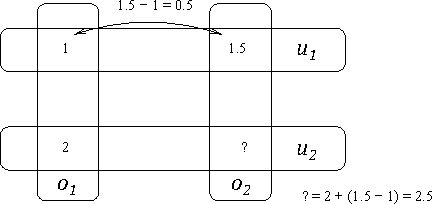
\includegraphics[width=0.7\linewidth]{slopeone.pdf}
  \caption{К объяснению работы алгоритма Slope One}
  \label{fig:slope-exp}
\end{figure}

При помощи данного алгоритма рейтинги объекта $o_2$, в общем случае, вычисляются из оценок нескольких пользователей и относительно разных объектов.  Т.е. получается несколько рейтингов одного и того же объекта. В этом случае считается средневзвешенная оценка полученных рейтингов, где в качестве весового коэффициента выступает количество раундов оценивания, другими словами, <<сколько раз пользователь $u_i$ проголосовал за <<опорный>> объект $o_j$?>>


\subsection{Гибридные методы}
\label{sec:hybrids}

В статье [11] рассмотрена задача разработки алгоритмов оценивания лекционного материала. Авторами предложен алгоритм вычисления близости лекций (объектов), где каждая лекция характеризуется подмножеством некоторого набора значений (например, подмножеством авторов лекций относительно множества всех авторов). Базовый алгоритм реализует подход фильтрации содержания. Для алгоритма подобранны коэффициенты, при помощи которых можно объединять оценки различных атрибутов в одну общую оценку лекции. Наиболее значимыми атрибутами оказались «категории», «авторы», «языки», «название» и «описание». Цель -- синтезировать набор лекций фиксированной длины, рекомендованных для просмотра заданному пользователю, из фиксированного множества <<новых>>, не использованных в построении профилей пользователя и объекта.

Далее алгоритм дополняется предсказателем последовательностей лекций: заданы примеры последовательностей из трех лекций, требуется для последовательностей из двух предложить третью, четвертую и т.д. Последовательности лекций приобретены системой неявно, т.е. фиксируя просмотренные пользователем лекции. Алгоритм занял первое место в соревновании, причем со значительным отрывом от второго места. Производится внедрение результатов исследований в области анализа сигналов и предсказания последовательностей событий.


%Приложения рекомендательных систем

    В \cite{b12} создан рекомендательный сервис новостей посетителям сайта, время пересчета рекомендаций в котором на каждую тысячу новых записей в журнале WEB"=сервера составляет 1.5--2 с., что авторами заявлено как ресурс, функционирующий в режиме, близком к реальному времени. Для проекта Рамблер"=новости подобный результат является удовлетворительным, так как 1000 новых запросов к сайту делается за чуть большее время. В исследовании использован адаптированный алгоритм MinHash для идентификации записей журнала и неточного их сравнения. Целью работы было показать целесообразность применения NoSQL"=технологий для создания сервисов указанного качества.

    Важным свойством приведенной реализации является то, что задачи хранения и анализа данных удалось объединить с задачей предоставления доступа к результатам в единой системе, избежав накладных расходов на перемещение данных из одного источника в другой, что улучшило общую производительность сервиса. Кроме того, предложенный подход упрощает решение повседневных задач сбора статистики о взаимодействии пользователя с веб"=приложением путем анализа структурированных логов мощным языком запросов СУБД MongoDB.  В результате продемонстрировано, что применение NoSQL к решению подобного класса задач является весьма перспективным.

\subsection{Оценка релевантности рекомендаций}
\label{sec:rs-eval}

Как и любая система структуризации информации РС оцениваются с точки зрения степени корректности расчетов рекомендаций. Классическим подходом является пример из \cite{b13}, где рассматривается задача сравнительной оценки различных подходов к построению РС.  Эта оценка, RMSE, среднеквадратическое отклонение, выполняется при помощи формулы:
    \[
      \mbox{RMSE}=\sqrt{\frac{1}{|D|}\sum_{(u,o)\in D}(\hat{r}_{u,o}-r_{u,o})^2},
    \]
где $D$ -- множество пар пользователей $u$ и объектов $o$, $r_{u,o}$ -- оценка интереса объекта $o$ пользователем $i$, \(\hat{r}_{u,o}\) -- оценка интереса, сделанная РС. Другие оценки представлены в \cite{b10}. % Nefedova




\section{РС для рынка недвижимости}
\label{sec:ex-retail}


В [18] предложен проект системы управления недвижимым имуществом, где варианты объектов предлагаются на основе вывода на прецедентах (case-based reasoning). Задача подсистемы вывода – найти  прецедент в базе имеющихся прецедентов, похожий на запрос пользователя. Система помогает покупателям найти имущество, соответствующее их запросам. При этом система выводит суждения о свойствах объектов. Полученная информация затем используется в процессе фильтрации содержания и коллаборативной фильтрации. В дополнение к полученному списку выводится также наиболее популярные (most visited) варианты.

В теоретическом исследовании [15] в системе пользователи разделены на продавцов и покупателей. Продавцы "рекламируют" свое имущество, выставленное на продажу, выделяя те свойства недвижимости, которые сами считают важными. Предложена идея того, как получать данные для фильтрации содержания в задаче разработки РС управления имуществом: продавцы выступают в виде экспертов-оценщиков недвижимости, формируя информационную базу для фильтрации содержания. Предложенную идею можно дополнить, если ввести третий класс пользователей - экспертов-риелторов и позволить им дополнять базу данных прецедентов новыми суждениями.

В [16] опытным путем показано, что использование Интернета не влияет значительно на эффективность поиска недвижимости с целью ее покупки по критериям времени поиска, его гибкости и "удовлетворенность результатом". Согласно исследованию Национальной ассоциации риелторов, проведенном в 2011 году, показано, что 88\% покупателей выбрали Интернет в качестве основного источника информации, но при этом среднее время на поиск жилья составило 12 недель, оно оказалось сравнимым с измерением, проведенным в 2009 году. Пользователь просматривает больше информации (как объектов, так и их свойств), но на анализ этой информации так же тратится много времени. Для повышения скорости выдачи результата авторами разработан алгоритм поиска на основе анализа поведения пользователей в процессе поиска объекта недвижимости, а также WEB-система, основанная на прецедентном выводе и онтологической концептуальной модели предметной области, ориентированная на пользователя.

В [23] авторами выделены три ключевые характеристики объекта недвижимости, которые в значительной мере является определяющими в процессе принятия решения – это "расположение" (location), "потребительская характеристика" (housing unit property) и "цена" (price). Большинство РС используют именно эти характеристики для фильтрации содержания, причем для критерия "потребительская характеристика" задаются формальные параметры объекта (площадь, номер этажа, количество балконов, комнат-спален и т.п.). На окончательное решение также влияет окружение объекта - расстояние до магазинов, школ, детских садов. Для того, чтобы учесть эти характеристики в [16] построена онтологическая модель, связывающая различные характеристики недвижимости в три древовидные структуры, описывающие варианты терминов "расположение", "потребительская характеристика" и "цена". Например, как вариант, под "расположением" понимается "расстояние" до места работы "пешком", выраженное в минутах. Так же "расположение" - это наличие в "окружении" (environment) объекта недвижимости "услуг" "фитнеса". При помощи онтологии получена возможность сравнивать не вполне "схожие" объекты, что повышает точность обработки информации.
Важным достижением авторов [16] является разработанный прототип РС, в котором пользователю предоставляется возможность указать на карте города область (окружность с заданным радиусом), в которой он хотел бы приобрести объект недвижимости, уточнить его потребительские характеристики и возможный диапазон цен.

Затем система выводит на карту варианты объектов недвижимости. Далее пользователь может уточнить другие характеристики, тем самым сужая количество предоставляемых вариантов. В сравнении с сервисами, подобным Avito.ru [17], пользователю предлагается меньше вариантов, т.е. система оценивает интерес пользователя более точно, и сильнее сужает количество альтернатив.
В [18] решается сложная логистическая задача организация процесса управления имуществом, в который вовлечены разнообразные группы людей в изменяющихся деловых и экономических условиях. В оценке учитываются не только экономические и бизнес-критерии, но и такие критерии, как "технологичность", "комфорт", "пространство", "административные" и "технические". Основная цель исследования - разработать модель, в которой различные группы людей будут максимально удовлетворены в "рациональной микро- и макро-среде".

Эффективность использования имущества предлагается оценивать по целой системе критериев, включающей цену объекта, цену владения этим объектом, цену ремонта, возможности его использования (capasity), количеству операций, которые необходимо выполнить по передаче собственности, надежность, комфорт, срок физической и технической эксплуатации, и др. Авторы разрабатывают математический аппарат для оценивания каждого объекта недвижимости – цены, эргономики, стоимости ремонта, назначение и т.п. Математическое обеспечение РС предложено развивать в направлении ухода от поиска <<наиболее экономически выгодного управления недвижимостью>> к мультикритериальному выбору и тем самым повысить эффективность вычислительных процессов.

\subsection{Коллаборативная фильтрация объектов недвижимости} % Такой прикольный заголовок теперь.
\label{sec:coll-filtering-rspo}
% На эту проблему обратил внимание Дедушка Ленин (Владимир Ульянов (Сергеевич)) в ИГУ на защите Пономарева.
% За что ему респект и уважуха.

Коллаборативная фильтрация в ее изначальной постановке эффективно применима для расчета оценок интереса к массовым товарам, которые приобретаются покупателями на интернет"=сайтах.  Объекты недвижимости -- это штучный товар и могут быть приобретены только одним покупателем. Поэтому выработка положительной оценки затруднена: невозможно интерпретировать факт покупки квартиры как положительную оценку. Причины тому две -- сайты продаж недвижимости не распространяют данную информацию, они только фиксируют факт наличие квартиры на рынке. Вторя причина (проблема) состоит в том, что если даже стало известно, что квартира куплена конкретным покупателем, эта квартира больше не участвует в оценивании другими покупателями.

Проблема в большей части решается следующим образом. Считать любое проявление некоторого интереса к объекту недвижимости со стороны покупателя положительной оценкой. Например, если покупатель выбрал квартиру из списка и занялся подробным ознакомлением с ее параметрами и фотографиями, считать, что данный объект представляет некоторый интерес.

Вторым подходом к применению метода коллаборативной фильтрации к объектам недвижимости -- это проводить оценку не отдельных объектов недвижимости, а из классов.  Для этого надо реализовать в РС подсистему анализа схожести объектов недвижимости (их атрибутов) и разделении их на некоторые классы. И если покупатель заинтересовался объектом из некоторого подмножества (кластера), то положительную оценку получает этот весь класс. Внутри класса объекты недвижимости можно считать равноценными.

Таким образом, применение одной лишь коллаборативной фильтрации для выработки рекомендаций и <<борьбы>> с <<холодным стартом>> в РС рынка недвижимости невозможно, поэтому, необходимо дополнят ее другими методами и подходами, что автоматически переводит такие РС в класс гибридных.

\subsection{Сопутствующие технические задачи}
\label{sec:co-tasks}

Одной из важных задач, решаемых при разработке РС, является создания пользовательского интерфейса, адекватно отображающего систему критериев, ко которым необходимо производить подбор объектов для пользователя. Например, в статье \cite{b14} представлен модуль естественно"=языкового интерфейса к базе данных РС, который реализован на основе математических моделей семантических объектов. При помощи модели решаются задачи определения семантики языковой конструкции, заданной пользователем, включая синонимы, классы, отношения и ограничения. В статье приводятся сведения о программной реализации предложенного метода в среде PHP~+~SQL и результатах тестирования программы на задаче доступа к базе данных РС автомобильного салона.

В \cite{b15} решается проблема обеспечения ограничения доступа к личным данным пользователей в контексте построения РС встраивания рекламных сообщений в информационный поток. При этом необходимо контролируемо предоставлять в одностороннем порядке в РС информацию из БД пользователей. Предложено вместо традиционных средств VPN (\foreignlanguage{english}{Virtual private network}) использовать режим функционирования сети с синхронным изменением IP"=адреса сервера и переключение клиента на этот адрес.

% РС (анализа, оценки и т.п.).

Кроме того, на современном этапе развития РС важными вопросами, решаемыми в процессе проектирования РС объектов недвижимости являются:
\begin{itemize}
\item разработка концептуальной модели предметной области в виде онтологии;
\item создание математических моделей предсказания значений атрибутов, описывающих объект недвижимости;
\item реализация механизмов компьютерного обучения и логического вывода на основе прецедентов;
\item обеспечение информационного наполнения РС для оценки качественных атрибутов (например, наличия школ и магазинов в шаговой доступности).
\end{itemize}
Решение данных задач в значительной мере влияет на качество и точность предсказания оценки значимости объекта недвижимости для пользователя.


\section{Среда программирования .NET}
Средой разработки веб-приложения выбран .NET/Mono как некоторый компромисс между производительностью реализации программного кода и производительностью его исполнения, а также богатым набором программных пакетов.

.NET Framework - программная платформа, выпущенная компанией Microsoft в 2002 году. Основой платформы является общеязыковая среда исполнения Common Language Runtime (CLR), которая подходит для разных языков программирования. Функциональные возможности CLR доступны в любых языках программирования, использующих эту среду.

Mono - проект по созданию полноценного воплощения системы .NET Framework на базе свободного программного обеспечения. Он обеспечивает практически полную переносимость кода и среды исполнения для стандарта~.NET версии~4.65.


\section{Технология Entity Framework}

Entity Framework представляет объектно"=ориентированную технологию на базе среды программирования .NET, которая обеспечивает объектно"=ориентированное представление реляционных данных. Если традиционные средства ADO.NET позволяют создавать подключения, команды и прочие объекты для взаимодействия с базами данных (БД), то Entity Framework представляет собой более высокий уровень, который позволяет абстрагироваться от реляционных свойств базы данных и получать доступ к данными независимо от типа хранилища \cite{entityframework}.

Первая версия Entity Framework -- 1.0 вышла в 2008 году и представляла библиотеку с небольшим набором функций, базовую поддержку ORM (object-relational mapping -- отображения данных на объекты) и один подход к взаимодействию с БД -- Database First. С выходом версии 4.0 в 2010 году Entity Framework стал рекомендуемой технологией для доступа к данным, а в сам фреймворк были введены новые возможности взаимодействия с БД -- Model First и Code First. Дополнительные улучшения функций среды последовали с выходом версии 5.0 в 2012 году. И наконец, в 2013 году был выпущен Entity Framework 6.0, обладающий возможностью асинхронного доступа к данным.

Центральной концепцией Entity Framework является понятие сущности или \verb|entity|. Сущность представляет набор данных, ассоциированных с определенным объектом. Поэтому данная технология предполагает работу не с таблицами, а с объектами и их наборами. Любая сущность обладает рядом свойств. Например, если сущность описывает человека, то мы можем выделить такие свойства, как имя, фамилия, рост, возраст, вес. Свойства необязательно представляют простые данные типа \verb|int|, но и могут представлять более комплексные структуры данных. Каждая сущность, как правило, описывается несколькими свойствами, которые отличают эту сущность от других и уникально ее определять. Подобные свойства играют роль ключей. При этом сущности могут быть связаны ассоциативной связью один-ко-многим, один-ко-одному и многие-ко-многим, подобно тому, как в реальной базе данных происходит связь через внешние ключи.

Отличительной чертой Entity Framework является использование запросов LINQ для выборки данных из БД. С помощью LINQ не только извлекаются из БД определенные строки, хранящие объекты, но и конструируются объекты, связанные различными ассоциативными связями.

Другим ключевым понятием является Entity Data Model. Эта модель сопоставляет классы сущностей с реальными таблицами в БД.
Entity Data Model состоит из трех уровней: \emph{концептуального},\emph{ уровень хранилища} и\emph{ уровень сопоставления} (отображения, mapping). На концептуальном уровне происходит определение классов сущностей, используемых в приложении. Уровень хранилища определяет таблицы, столбцы, отношения между таблицами и типы данных, с которыми сопоставляется используемая база данных. Уровень сопоставления служит посредником между предыдущими двумя, определяя сопоставление между свойствами класса сущности и столбцами таблиц. Таким образом, через классы, определенные в приложении, обеспечивается взаимодействие с таблицами из базы данных.

Рассмотрим пример определения новой сущности в БД, поддерживаемой Entity Framework. В качестве объекта создадим пользователя:
\begin{minted}{csharp}
public class User
{
    public int Id { get; set; }
    public string Name { get; set; }
    public int Age { get; set; }
}
\end{minted}
Это обычный класс, который содержит некоторое количество свойств. Каждое свойство будет сопоставляться с отдельным столбцом в таблице БД.

Надо отметить, что Entity Framework в режиме Code First требует определения ключа элемента для создания первичного ключа в таблице в БД. По умолчанию при генерации БД среда в качестве первичных ключей рассматривает свойства с именами \verb|Id| или \verb|[Имя_класса]Id| (то есть \verb|UserId|).

Для взаимодействия с БД нам нужен контекст данных, т.е. среда, при помощи которой осуществляется создание экземпляров, в данном случае, пользователей, их запись в БД, механизмы транзакций, модификация объектов и т.п.

\section{Библиотека Brightstar DB}
В качестве контекста в данном проекте выступает база данных, реализованная на основе библиотеки Brightstar DB.

BrightstarDB является уникальной технологией хранения данных для платформы .NET. Она сочетает в себе гибкость, масштабируемость и производительность, а таже позволяет создавать приложения, используя знакомые инструменты разработчиков.
Ассоциативная модель

BrightstarDB построен на гибкой модели ассоциативных данных -- RDF. Граф RDF позволяет представлять все существующие, имеющие практический смысл, виды моделей данных. Модель основана на концепции троек. Каждая тройка -- это ассоциация некоторого  свойства с определенным ресурсом или значением. Модель позволяет описывать и представлять данные любой структуры высокого уровня, что создает средства разработки систем, эволюционирующих во времни, и комплексных систем на основе объединения данных различной природы.

BrightstarDB находдится среди немногих NoSQL\;--\;баз данных, предлагающих механизмы, <<понимающие>> описания структур данных, что позволяет им автоматически управлять отношениями между сущностями. Большинство NoSQL\;--\;баз данных требуют от разработчиков, чтобы он сам заботились об обновлении связей между документами и хранении дополнительных данных в хранилищах, отображающих ключи на значения. Базы данных NoSQL не особо хорошо справляются со моделями данных реальных приложений, таких как социальные сети или обработка графов.

BrightstarDB, будучи NoSQL\;--\;базой данных, поддерживает технологии Семантического веба. Она может использоваться как встроенная библиотека или как служба на сервере. К серверу обеспечивается сетевые соединения по протоколам HTTP, TCP/IP и через поименованные каналы. BrightstarDB обеспечивает поддержук Entity Framework в режиме Code First. Инструментарий, совместимый с Entity Framework также порождает объектный контекст при помощи задаваемых разработчиком .NET-приложений интерфейсов хранимых объектов в BrightstarDB.

%Хранение данных без хранения схемы данных
Используемая ассоциативная модель позволяет добавлять новые данные в базу данных BrightstarDB без традиционной необходимости определения схемы данных. Это еще больше повышает гибкость и поддерживает эволюционную разработку проектов, которая является важнейшей особенностью именно современных программных решений. Хранилище без схемы данных, реализованное в BrightstarDB, позволяют импортировать данные любой формы, а также связывать их друг с другом. Но и типизированые строго определенные структуры объектов также хорошо поддерживаются BrightstarDB. Разработчикам приложений, таким образом, можно отображать несколько моделей в .NET и в нескольких базах данных BrightstarDB.
%Модель данных со схемой

%Автоматическое кэширование данных

Результаты запросов и представления кэшируются автоматически для повышения производительности приложений с интенсивным использованием запросов к БД. Как правило, кэширование данных производится самими приложениями, т.е. реализуется разработчиком как отдельный функциональный блок, но BrightstarDB обеспечивает эту функцию как ключевую возможность.
%Поддержание истории изменений

BrightstarDB использует форматы хранения данных, которые сохраняют полную информацию об истории на каждом этапе транзакции. Это позволяет приложениям выполнять запросы данных в любой момент времени. Обеспечивается проверка состояния данных в хранилище данных, а также  возврат в предыдущее состояние или снимок (snapshot), если ранее он был сделан. Такой подход конечно увеличивает объем используемого дискового пространства, но BrightstarDB предоставляет и возможность консолидировать данные, относящиеся только к текущему моменту времени.
% Инструментарий, дружелюбный к разработчику

Большинство разработчиков на .NET привыкли использовать объекты и LINQ для построения приложений. LINQ поддерживается практически в полной мере, включая типизированную модель данных.  Причем, множество различных объектных моделей могут налагаться друг на друга в общей семантической модели данных. В BrightstarDB существует поддержка языка запросов SPARQL, а также экспорт/импорт данных в формате NTriples, используемые при построении семантических веб-приложений. В большинстве ORM изменения в объектной модели и в реляционной схеме должны осуществляться одновременно. RDF, в идеале, может быть использован для хранения и свойств-значений и отношений между объектами. Если объектная модель изменяется, то новое значение свойства может быть просто добавлено, так как нет фиксированной схемы. Аналогичным образом, если дополнительные данные добавляется в хранилище в виде RDF, то объектная модель может либо их игнорировать, либо использовать эти данные.

BrightstarDB является СУБД с однократной записью, многократным чтением (WORM). Изменения в данные добавляются в конец файла хранилища, данные никогда не перезаписываются.  Так как запись производится только одним клиентом, и данные не перезаписываются, то нет и необходимости в реализации блокировок. WORM-подход поддерживает откат и запросы по всей истории состояний базы данных на любом этапе транзакции. База данных может периодически консолидироваться, при этом происходит удаление ненужной истории, и это позволяет управлять ростом размера файла хранилища.

База данных РС создана на основе технологий семантического веба, реализованных в программном пакете BrightStarDB. Данные хранятся в виде графа, к графу реализован объектно"=ориентированный доступ по стандарту Entity Framework. При этом обеспечивается как удобный инструмент реализации приложения, так и перспектива расширения методов анализа данных интеллектными методам на основе концептуальной модели предметной области.

\section{Библиотека Nancy для создания интернет-приложений}

Для реализации системы отслеживания действий пользователя на сайте в данном приложении был выбран фреймворк NancyFX. Главное преимущество данного фреймворка заключается в том, что маршрут, т.е. сам запрос определяется в конструкторе модуля. Чтобы определить маршрут в NancyFX, необходимо указать Method (Метод) + Pattern (Шаблон) + Action (Действие).
Method (Метод) – это метод HTTP, который используется для доступа к ресурсу. Nancy поддерживает следующие методы: DELETE, GET, HEAD, OPTIONS, POST, PUT и PATCH.

GET - запрашивает данные из указанного ресурса; POST - отправляет данные, подлежащие обработке, на указанный ресурс; PUT заменяет все текущие представления ресурса данными запроса; DELETE удаляет указанный ресурс; HEAD - запрашивает ресурс так же, как и метод GET, но без тела ответа; OPTIONS - используется для описания параметров соединения с ресурсом; PATCH - используется для частичного изменения ресурса;

Pattern (Шаблон) - объявляет URL-адрес приложения на который отвечает маршрут.

Action (Действие) - это поведение, которое вызывается, когда запрос сопоставляется с маршрутом.

Для примера можно привести следующий запрос:

\begin{pzlisting}
\caption{Пример \protect\textsc{GET}-запроса на NancyFX}
    \begin{minted}[mathescape,linenos]{csharp}
    public class HelloNancyFx : NancyModule
    {
        public HelloNancyFx()
        {
            Get["/"] = parameters => "Hello, NancyFX!";
        }
    }
\end{minted}
\end{pzlisting}
В конструкторе данного класса есть строка 5, в которой реализуется GET"=запрос, соответствующий корню сайта в браузере. В результате пользователю выдается сообщение <<Hello, NancyFX!>> в виде простого (plain) текста. Библиотека Nancy разрабатывалась как негромоздкий способ реализации функций интернет-приложения, более понятный и простой в отличие от ASP.NET. Кроме этого, NancyFX работает на Mono. % На самом деле они оба на моно работают.

Приложение Nancy строится как набор таких отображений вида \verb|GET["<адрес>"]|, \verb|POST["<адрес>"]| и т.д. При этом \verb|<адрес>|, в общем случае, содержать структуры вида \verb|"<адрес>/{var}"|, где \verb|var| -- это динамическая переменная C\#, куда поместится строка, стоящая в адресе после <<\verb|/|>>. Доступ к \verb|var|, к данным формы, к параметрам \verb|GET|- и \verb|POST|-запросам и т.п. передается через переменную \verb|parameters| и \verb|public|-атрибут \verb|Request|. Например, данные формы доступны в \verb|Request.form.<имя_поля>|.

Результатом запуска методов HTTP является возвращаемый объект \verb|Response|, кодирующий ответ сервера в том числе и передаваемый клиенту гипертекст. При помощи данного объекта также осуществляется управление браузером пользователя, например, переадресация на другую страницу, хранение куки и т.п.  Для генерирования гипертекста в Nancy реализован ряд механизмов заполнения шаблонов данными (шаблонизаторов). Но можно также подключать и другие технологии, в частности \textsc{SharpTAL}.


\section{Библиотека SharpTAL для создания HTML-страниц}
В проекте использован шаблонизатор \textsc{SharpTAL}, обладающий рядом важных преимуществ, в том числе, строгой изоляцией исполняемого кода от описания HTML-шаблона; все вычислимые конструкции встраиваются внутрь XML-атрибутов, не влияя на базовую спецификацию XML (HTML), в которой представлен шаблон.  Рассмотрим пример шаблона, представленного в листинге~\ref{lst:TAL}.

\begin{pzlisting}
  \caption{Шаблон \textsc{SharpTAL} (пример)}\label{lst:TAL}
\begin{minted}[linenos]{xml}
<html>
  <body>
    <h1>Hello, ${"world"}!</h1>
    <table>
      <tr tal:repeat='row new string[] {"red","green","blue"}'>
        <td tal:repeat='col new string[] {"rectangle","triangle"}'>
           ${row} ${col}
        </td>
      </tr>
    </table>
  </body>
</html>
\end{minted}
\end{pzlisting}

Для генерирования текста по этому шаблону нужно в параметры функции-интерпретатора передать шаблон и параметр -- отображение имени на объект C\#.  В данном примере необходимо задать значение переменной \verb|world|, которое, является или строкой или должно поддерживать интерфейс преобразования к строковому значению.  В строках 5 и 6 листинга~\ref{lst:TAL} задается ва вложенных цикла, при помощи которых генерируется декартово произведение двух множеств объектов. Значения передаются в переменные цикла \verb|row| и \verb|col|.  Циклы в шаблоне задаются при помощи TAL-выражений \verb|tal:repeat|, структура этого выражения следующая:
\begin{center}
\verb|<переменная_цикла> <выражение C#>|,
\end{center}
причем \verb|<выражение С#>| должно возвращать список значений или объект, поддерживающий интерфейс \verb|IEnumerable|.

Подсистема веб-сервера сконструирована на основе пакетов Nancy и SharpTAL. На основе xUnit создан сервис тестирования функционирования приложения.

\section{Идентификация сеанса пользователя в HTTP}

Для того, чтобы пользователю давать наиболее адекватную рекомендацию, необходимо связать каждый сеанс взаимодействия пользователя с сайтом в один общий сеанс.  Данная техническая проблема решается двумя способами. Первый способ -- это разработать систему регистрации пользователей на сайте, второй -- связать отдельные сеансы при помощи так называемых \emph{записей куки}.  Первый способ требует от пользователя проявить желание зарегистрироваться, и каждый раз как пользователь будет регистрироваться на сайте старые данные будут дополняться новыми. Для обеспечения функционирования сеансов с регистрацией также используются куки.

Второй способ позволяет создавать пользовательские учетные записи, привязанные только к куки. Рассмотрим использование куки на примере.  Для доступа к странице http://www.example.org/index.html, браузер отправляет на сервер www.example.org следующий запрос (браузер → сервер):
\begin{minted}{http}
GET /index.html HTTP/1.1
Host: www.example.org
\end{minted}
Сервер отвечает, отправляя запрашиваемую страницу вместе с текстом, содержащим HTTP-ответ. Там может содержаться указание браузеру сохранить куки(браузер ← сервер):
\begin{minted}[linenos]{http}
HTTP/1.1 200 OK
Content-type: text/html
Set-Cookie: name = value

<Содержимое страницы>
\end{minted}

Поле \verb|Set-cookie:| (строка 3) отправляется лишь тогда, когда приложение на сервере сообщает браузеру команду на сохранение куки-значений. В этом случае, если куки поддерживаются браузером и их приём включён, браузер запоминает строку \verb|name=value| и отправляет её обратно серверу с каждым последующим запросом. Например, при запросе следующей страницы \verb|http://www.example.org/spec.html| браузер пошлёт серверу \verb|www.example.org| следующий запрос (браузер → сервер):
\begin{minted}[linenos]{http}
GET /spec.html HTTP/1.1
Host: www.example.org
Cookie: name = value
Accept: */*
\end{minted}

Этот запрос отличается от первого запроса тем, что содержит в строке 3 значения, которые сервер отправил браузеру ранее. Таким образом, сервер узнает, что этот запрос связан с предыдущим. Сервер отвечает, отправляя запрашиваемую страницу и, возможно, добавив новые куки. Значение куки может быть изменено сервером путём отправления новых строк \verb|Set-Cookie: name=newvalue|. После этого браузер заменяет старое куки с тем же name на новую строку.

Куки также могут устанавливаться программами на языках типа \textsc{JavaScript}, встроенными в текст страниц, или аналогичными скриптами, работающими в браузере. В \textsc{JavaScript} для этого используется свойство \verb|cookie| объекта \verb|document| -- \verb|document.cookie|. Например, \verb|document.cookie = "temperature=20"| создаст куки под именем «temperature» и значением 20.

Преимущества значений куки:
\begin{itemize}
\item Их очень легко использовать и реализовать;
\item За отсылку данных отвечает браузер;
\item Браузер автоматически сохраняет файлы куки посещаемых сайтов.
\end{itemize}
Ограничения технологии куки:
\begin{itemize}
\item данные хранятся в простом текстовом формате, поэтому никакая
  безопасность не гарантируется;
\item ограничения на объем
  памяти данных значений --  4096 bytes (4KB);
\item число хранимых значений ограничено, многие браузеры предоставляют возможность хранить 20
  значений куки, и если будет отослан новое значений куки, то старое будет
  удалено; некоторые браузеры поддерживают до 300 значений куки.
\end{itemize}


Значения куки разделяются на два типа:
\begin{itemize}
\item Постоянные куки;
\item Сеансовые куки или временные;
\end{itemize}

\emph{Сеансовые куки} действуют на время работы пользователя с сайтом (активного сеанса) и хранятся в оперативной памяти активного процесса браузера.

В отлитие от сеансовых куки \emph{постоянные куки} хранятся на клиентском жестком диске до тех пор, пока не истечет их срок хранения, который задается специальным образом. Обычно -- это конкретная дата. Кроме того, куки могут быть удалены пользователем, для этого в браузерах есть специальные инструменты. Постоянные куки -- это основной инструмент сбора определенной информации о пользователе и его операционной системе.

\paragraph{Выводы по разделу.}

Рекомендательные системы (РС) позволяют структурировать объекты в базе данных информационного ресурса (интернет-магазина) по степени релевантности к интересам того или иного пользователя (категории пользователей). Они позволяют решать задачи поиска новых закономерностей в таких данных, новые свойства и характеристики объектов.

РС активно применяются в интернет-магазинах, библиотеках текстового содержания (цифровых архивов статей научного учреждения или проекта, книг), а также на рынках недвижимости.

В области РС существует ряд фундаментальных и практических проблем, требующих решения как на этапе разработки РС, так и на этапе их эксплуатации:
\begin{itemize}
\item пользователи неохотно предоставляют информацию о себе и
  своих потребностях, либо разработчики РС уделяют мало внимания
  процессу информационного наполнения профиля пользователя;
\item в предметных областях, связанных с большой стоимостью объекта или услуги (где принимается серьезные решения по вложения материальных средств), информационные модели объекта и профиля пользователя сложны по своей структуре и связи компонент структуры, что требует явного представления концептуальной модели предметной области во время выполнения РС как своих основных функций, так и функций предсказания значений атрибутов объекта или профиля пользователя на основе прецедентов;
\item для предыдущего пункта важным является также разработка пользовательского интерфейса, позволяющего в удобной для пользователя форме и достаточно гибко задавать запросы к РС, а также визуализировать результаты, предлагаемые РС;
\item при практической реализации РС практически всегда необходимо решать проблему <<холодного старта>>, т.е. обеспечивать функционирование информационной системы в режиме недостатка исходных данных о предпочтениях пользователей.
\end{itemize}

Таким образом РС, как системы поддержки принятия решения, являются типичным представителем систем \emph{искусственного интеллекта}, ориентированными, прежде всего, на обработку неполной и противоречивой информации, а также использующими системы, основанные на формализованных знаниях (\foreignlanguage{english}{knowledge-based systems}). Рекомендательные системы реализуются, как правило, в виде интернет-приложений, чтобы обеспечить максимальную доступность пользователю необходимой информации.

\chapter{ПРОЕКТИРОВАНИЕ И РЕАЛИЗАЦИЯ РЕКОМЕНДАТЕЛЬНОЙ СИСТЕМЫ}
\label{chap:dev-tech-theory}
\section{Функциональное моделирование предметной области}

Перед тем, как начать разработку программного продукта необходимо провести исследование предметной области автоматизации, на первом этапе, -- это узнать какие функции должен будущий программный продукт выполнять.

На рисунке~\ref{fig:umlusecase} изображена диаграмма UML <<Варианты использования>> (Use Case).  С РС взаимодействуют пользователи, которым можно присвоить три роли: <<покупатель>>, <<риелтор>> и <<эксперт>>. Все функции, доступные для покупателя доступны и для риелтора и для эксперта. Для выявления функций произведен опрос пользователей.  Задавались вопросы о том, какие действия выполняют пользователи (риэлторы и покупатели) совершают, чтобы достичь своих целей на сайтах продажи недвижимости. Роль эксперта появилась вследствие необходимости реализации функций кластерного анализа, что в свою очередь обусловлено невозможностью прямого применения метода коллаборативной фильтрации к решению данной задачи (см.~раздел~\ref{sec:collab-filtering-rspo}).
\begin{figure}[htbp]
  \centering
  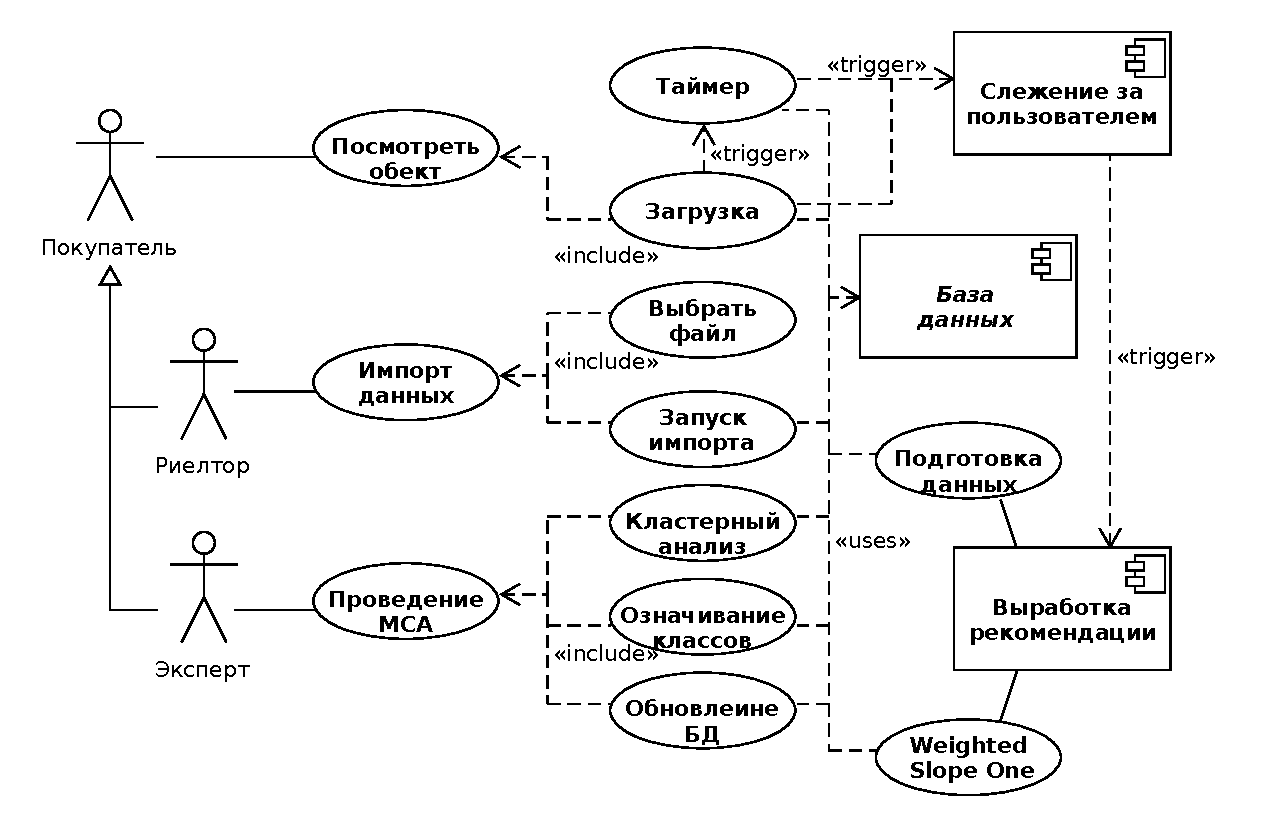
\includegraphics[width=0.9\linewidth]{use_case.pdf}
  \caption{UML-Диаграмма вариантов использования}
  \label{fig:umlusecase}
\end{figure}

Покупатель, находясь на сайте РС, может просматривать объекты недвижимости.  Для того, чтобы выдать информацию пользователю необходимо загрузить данные из базы данных. В это время информационная система собирает дополнительную информацию о том, интересен ли данный объект покупателю. Если пользователь находится на странице больше некоторого порогового значения времени, то система делает предположение, что покупатель положительно оценил данный объект недвижимости. Реализуется эта функция при помощи функции таймера, которая запускается в момент отображения страницы пользователю.

Если покупатель не покинул страницу в течение некоторого времени, то производится запись в базу данных о <<положительной оценке>> данного объекта, после чего запускается процедура пересчета оценок других объектов в данном классе объектов недвижимости. Предложенный вариант функционирования основывается на умозрительном предположении, что покупателей интересуют только объекты недвижимости одного класса.

Роль риелтора дополняется функцией загрузки исходных данных об объектах недвижимости в базу данных РС. Процедура состоит из трех шагов. Сперва надо скачать базу данных с сайта продажи недвижимости, например, с \url{http://atlcom.ru/} (Атлант-недвижимость), и поместить информацию в файл.  Затем, на втором шаге, надо выбрать этот же файл для загрузки в РС.  Третий шаг -- это запуск выполнения процесса загрузки данных.

Роль эксперта -- это структуризация данных базы данных, которая, как правило, проводится после загрузки данных риелтором. Функции эксперта включают проведение кластерного анализа данных, что формирует начальное распределение объектов недвижимости по классам, и сами эти классы.  Следующей функцией эксперта является <<Означивание классов>>.  При помощи этой функции эксперт просматривает элементы каждого кластера, проводить визуальный анализ (например, сравнение объектов друг с другом), и задавать имена кластерам. Два кластера, обозначенных одним и тем же названием, объединяются в РС в один общий кластер, и дальнейшая обработка информации уже производится в рамках этого объединенного множества объектов недвижимости.  Так же эксперт может редактировать накопленные значения оценок в базе данных. % Эта функция не реализована.

В системе реализованы два программных \emph{агента}. Агентами являются подсистемы, которые запускаются при возникновении некоторых событий, например, по факту попадания положительной оценки в базу данных, по факту просмотра пользователем объектов заданного кластера, а также вследствие действий эксперта.

Первый агент -- это механизм слежения за пользователем, который запускается таймером на странице веб-браузера. Второй программный агент -- это механизм пересчета оценок непросмотренных объектов, который запускается первым агентом или экспертом. Разделение этих агентов обусловливается тем, что не всякое срабатывание таймера должно обязательно запускать выработку рекомендаций, так как это процедура вычислительно емкая.  Другой причиной является потенциальное разделение процессов работы сервера, слежения за пользователем и пересчета рекомендаций по разным ядрам микропроцессора сервера. Такое разделение преследует целью повысить скорость отклика системы за счет утилизации всех ресурсов процессора.

\section{Архитектура системы}
Архитектура системы (рисунок~\ref{fig:architecture}) реализует общую клиент"=серверную схему взаимодействия интернет"=приложений.
\begin{figure}[htbp]
  \centering
  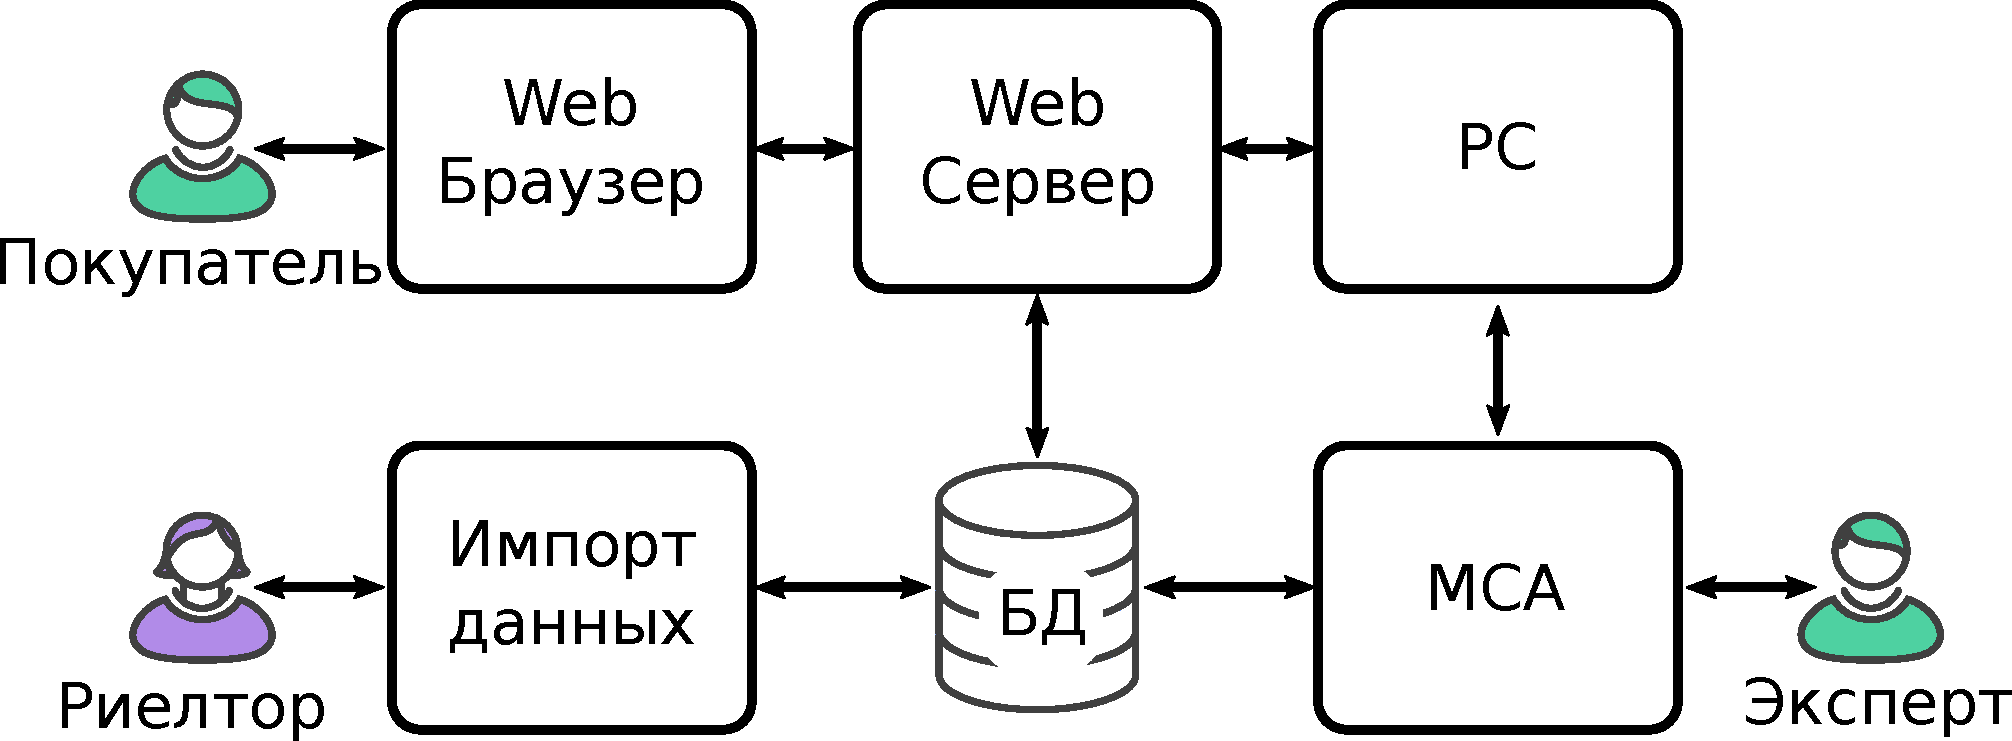
\includegraphics[width=0.7\linewidth]{architecture.pdf}
  \caption{Архитектура рекомендательной информационной системы}
  \label{fig:architecture}
\end{figure}

Предложения по недвижимости импортируются риелтором или администратором, которые хранятся в базе данных сайта типа Avito.ru. Пользователь взаимодействует с рекомендательной системой через веб"=браузер (клиентская часть), а веб"=сервер отвечает за хранение, обработку и преобразование информации к виду, воспринимаемому пользователем. База данных (БД) взаимодействует с блоком многомерного статистического анализа (МСА) данных, в котором находятся функции оценки схожести объектов, кластерный анализ и др. В рекомендательной системе (РС) находятся функции выработки рекомендаций для пользователя, рекомендации которой представляются в виде веб"=страницы и передаются Web-сервером Web-клиенту.

\section{Проектирование структуры базы данных}

\begin{figure}[htbp]
  \centering
  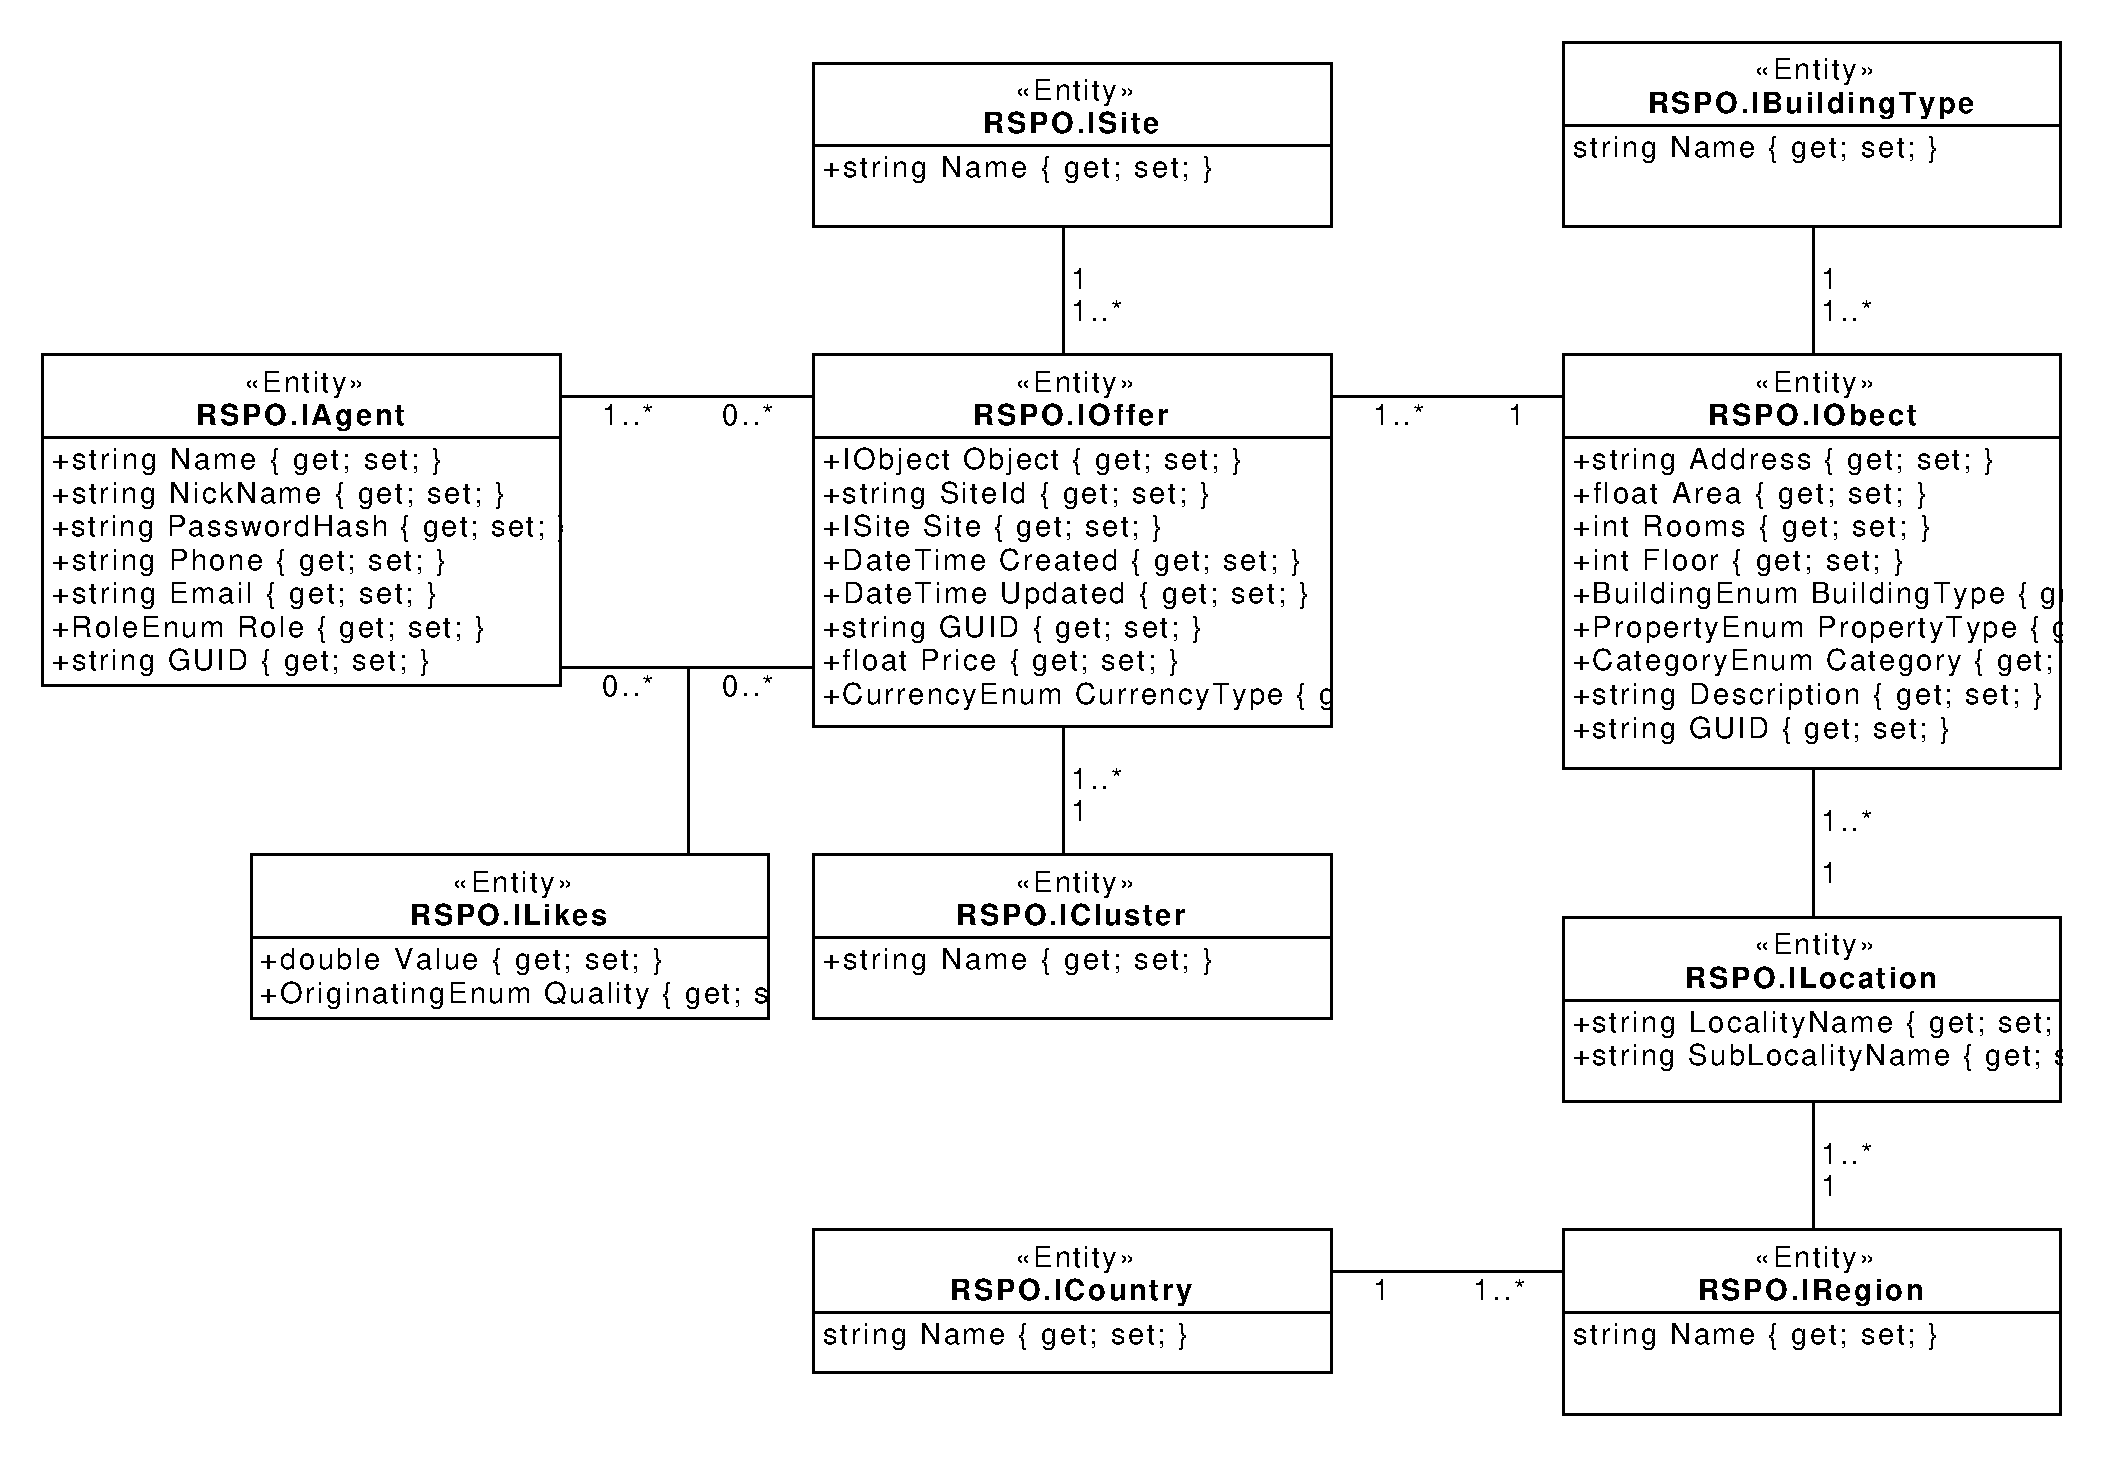
\includegraphics[width=0.9\linewidth]{class_diagram.pdf}
  \caption{Диаграмма классов рекомендательной системы (база данных)}
  \label{fig:classdiagram}
\end{figure}

\section{Импорт данных в хранилище}

Особенностью рынка недвижимости является тот факт, что актуальные данные об объектах недвижимости опубликованы в свободном доступе: разработаны специальные форматы обмена данных и API"=интерфейсы сайтов для доступа к этим данным. Ввиду достаточно высокой универсальности эти данные не содержат каких"=либо характеристик релевантности к интересам клиентов.


\subsection{Источники информации}
\subsection{Обменный формат данных}
\subsection{Подсистема импорта данных}
\section{Проектирование интернет-приложения}
\subsection{Серверная поддержка протокола HTTP}
\section{Реализация подсистемы рекомендаций}
\subsection{Подсистема слежения за пользователем}
Поэтому основной функцией разрабатываемого веб"=приложения являются сбор информации об интересах пользователя: пользователь, находясь на сайте и просматривая перечень объектов, сообщает системе свои намерения. РС, затем, производит анализ полученных данных и относит пользователя к тому или иному классу. Рекомендации строятся в виде подмножеств объектов, просмотренных пользователями данного класса, т.~е. на основе метода коллаборативной фильтрации.

2.4.	Идентификация пользователя
При первом подключении к сайту, пользователю присваивается уникальный идентификатор GUID и куки, если пользователь уже зарегистрирован на сайте, то его GUID и являются куки. GUID используется абсолютно для всех пользователей, зарегистрированных или анонимных. GUID (Globally Unique Identifier) - это уникальный, статический 128-битный идентификатор. Главная особенность GUID – это его уникальность, которая позволяет создавать расширяемые сервисы и приложения без опасения конфликтов в случае совпадения идентификаторов. Хотя уникальность каждого отдельного GUID не гарантируется, потому что общее количество уникальных ключей настолько велико (2128), что вероятность того, что в мире будут независимо сгенерированы два совпадающих ключа, крайне мала. В момент подключения к сайту также создается и сессия для пользователя, которая при помощи метода protected Nancy.Response InSession(Nancy.IResponseFormatter response = null) добавляет текущую сессию в словарь всех сессий. При подключении к любой странице сайта производится GET- запрос в параметрах которого присутствует метод protected void RestoreSession(), который позволяет восстановить предыдущую сессию. Идентификация пользователя представлена на рисунке 15.


Рисунок 15. Идентификация пользователя


\paragraph{Создание сессии.}
При подключении пользователя к сайту, запрашиваются данные с помощью \verb|GET|-запроса на URL:\url{http://127.0.0.1:8888/}. Обработка ответа на \verb|GET|-запрос пользователя выглядит следующим образом:
\begin{pzlisting}
\caption{Создание сессии}
\begin{minted}[linenos]{csharp}
    Get["/"] = parameters =>
        {
            RestoreSession();
            ApplicationModel appModel =
                new ApplicationModel(Application.APPLICATION_NAME);
            return Render("index.pt",
                     context: appModel,
                     view: new ApplicationView(appModel,
                         CurrentSession));
        };
\end{minted}
\end{pzlisting}
В нём проверяется уникальный идентификатор GUID для пользователя в методе RestoreSession(); и если такой GUID уже существуют, то происходит восстановление предыдущей сессии со всеми запросами, которые делал данный пользователь на сайте, а также восстановление значение куки, так как GUID и являются куками для зарегистрированного пользователя. Далее более подробно рассмотрим метод protected void RestoreSession().

\paragraph{Восстановление сессии}
Метод \verb|protected void RestoreSession()| отвечает за восстановление сессии по кукам. При первоначальном подключении пользователя к сайту, ему присваивается пустое строковое значение \verb|string value = "";|, которое далее мы проверяем с помощью конструкции try-catch. В блоке try в значение value смотрим куки и если, они существуют в данном подключении, то восстанавливаем предыдущую сессию пользователя. В случае если значение оказывается пустым, то создаем новую сессию с присвоением GUID. Если пользователь зарегистрирован на сайте, то восстановление его сессии происходит с помощью GUID. При посещении сайта, пользователю отправляется GET- запрос:

Листинг 3. Восстановление сессии

% TODO: Взять сам RestoreSession

В котором проверяются его уникальный идентификатор GUID в методе RestoreSession(); далее мы ищем такой GUID в  базе банных и если такой GUID уже имеется, то происходит восстановление предыдущей сессии со всеми запросами, которые когда-либо делал данный пользователь на данном сайте.

\paragraph{Создание куки.}
Для создания сессии необходимо присвоить какой-нибудь уникальный идентификатора пользователю сайта, так как некоторые пользователи могут быть не зарегистрированы и для сохранения их результатов запроса необходимо использовать данные методы.
Для начала создадим метод, который будет присваивать куки для каждого пользователя, посетившего данный сайт:
% TODO: правильный код.
В нашем случае, срок хранения куки файлов составляет один год. Куки хранят информацию об аутентификации пользователя, персональные предпочтения и настройки пользователя, отслеживают состояние сеанса доступа пользователя. Далее рассмотрим, как происходит регистрация пользователя на сайте.

\paragraph{Регистрация пользователя.}
На сайте присутствует возможность регистрации пользователя. Данные, которые вводятся в поля регистрации пользователя, отвечает отдельный интерфейс IAgent. Рассмотрим IAgent подробнее.

\paragraph{Интерфейс IAgent.}
Интерфейс \verb|IAgent.cs| определяет основные свойства объектов, представляющих пользователя. По структуре этого интерфейса порождаются объекты \verb|Agent|, хранимые в EntityFramework\;--\;базах данных, в частности BrightstarDB. В листинге~\ref{lst:iagent} представлен подробно \verb|public interface IAgent|.
\begin{pzlisting}
\caption{Интерфейс регистрации пользователя}\label{lst:iagent}
\begin{minted}{csharp}
public interface IAgent
    {
        string Name { get; set; }
        string NickName { get; set; }
        string PasswordHash { get; set; }
        string Phone { get; set; }
        string Email { get; set; }
        RoleEnum Role { get; set; }
        string GUID { get; set; }
        [Ignore]
        bool Valid { get; }
    }
\end{minted}
\end{pzlisting}

\noindent\verb|string Name| – отвечает за имя пользователя,\\
\verb|string NickName| – логин пользователя,\\
\verb|string PasswordHash| – хэш пароля пользователя,\\
\verb|string Phone| – номер сотового телефона пользователя,\\
\verb|string Email| – электронная почта пользователя,\\
\verb|RoleEnum Role| – роль пользователя в системе: пользователь может зарегистрироваться как «Агент продаж», «Покупатель», <<Эксперт>>;\\
\verb|string GUID| – уникальный идентификатор пользователя;\\
\verb|bool Valid| – флаг анонимности пользователя.

После регистрации, пользователю выводится сообщение об успешной регистрации в системе. Для него создается новая сессия и  объект пользователя в сессии \verb|Session.Agent=agent;| и уникальный идентификатор его сессии \verb|Session.GUID = user.GUID;|. Все зарегистрированные пользователи хранятся в базе данных, список которых можно посмотреть, как представлено на рисунке~\ref{fig:userlist}.
\begin{figure}[htbp]
  \centering
  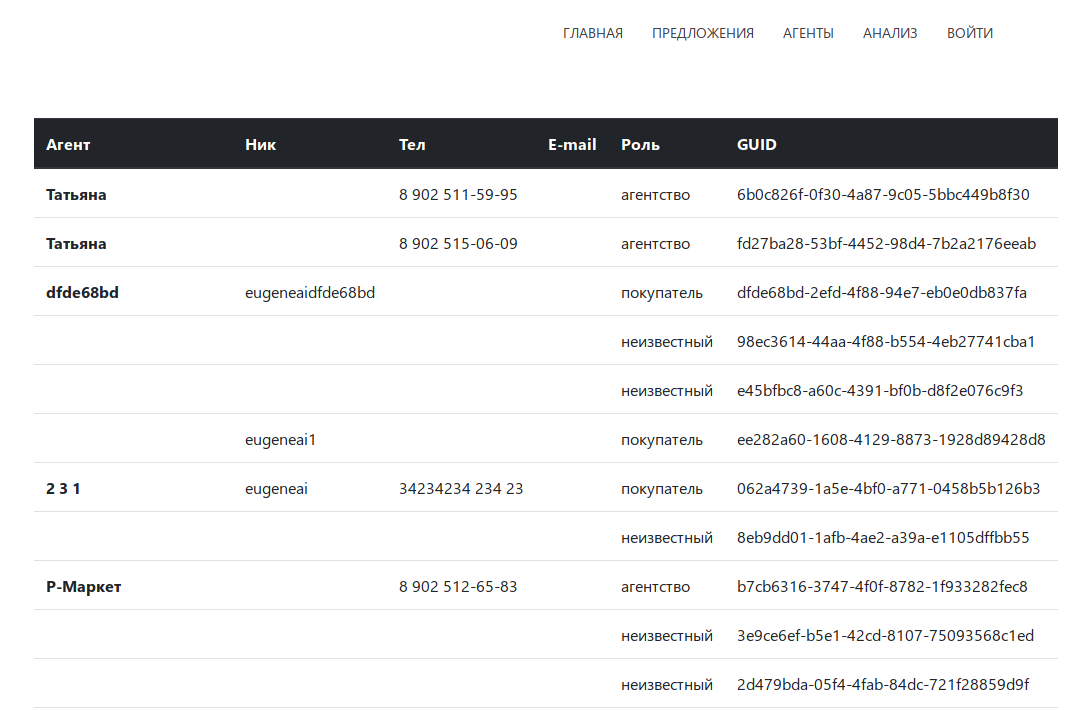
\includegraphics[width=0.8\linewidth]{screen-user-list.png}
  \caption{Список пользователей, включая анонимных}
  \label{fig:userlist}
\end{figure}
\paragraph{Объекты сессии}

\paragraph{Авторизация пользователя.}
Авторизация пользователя реализована в классе Server.cs, в методе public WebModule() : base()  с помощью POST-запроса, принимаем данные пользователя из формы регистрации и в случае успешной авторизации перенаправляем пользователя на домашнюю страницу сайта:

\begin{pzlisting}
\caption{Авторизация пользователя на сайте}
\begin{minted}{csharp}
    Post["/login"] = parameters =>
        {
            RestoreSession();

            LoginObject model = new LoginObject();
            LoginView view = new LoginView(model, this.Request, CurrentSession);

            Response response = null;
            bool res = view.Process();

            CurrentSession = view.Session;
            if (res)
            {
                response = Response.AsRedirect("/");
            }
            else
            {
                response = Response.AsRedirect("/login");
            }
            return InSession(response);
        };
\end{minted}
\end{pzlisting}

\subsection{Реализация алгоритма Slope One}
\subsection{Вычисление оценки объекта на основе гибридного подхода}
\subsection{Подсистема кластерного анализа}

Цель кластерного анализа -- это структуризация множества объектов по схожести. Как правило, такая структуризация преследует целью образование групп схожих между собой объектов, которые называются кластерами. \textbf{С помощью эмпирических данных которые накапливаются в базе данных системы, а также данных введенных пользователем, анализируются и обрабатываются алгоритмом агломеративного кластерного анализа, так как мы не можем изначально предлагать варианты недвижимости пользователю, не зная его интересов, нужно узнать с каким пользователем мы имеем дело. Поэтому используем кластерный анализ, предлагая пользователю разные варианты недвижимости из разных классов. Далее более подробно рассмотрим принцип агломеративного метода кластерного анализа.}

\paragraph{Агломеративный метод кластерного анализа.}
Агломеративный метод кластерного анализа предполагает, что каждый объект в начале исследования является отдельным кластером и производится группировка схожих объектов на основании матрицы мер сходства по кластерам. На заключительном этапе выполняется сохранение данных о кластеризации объектов. Вычисляются центры кластеров, каждому объекту присваивается свой номер кластера для дальнейшего использования кластеров при автоматизированных расчетах без повторной кластеризации данных.

Агломеративный метод кластерного анализа характеризуется последовательным объединением исходных элементов и соответствующим уменьшением числа кластеров. В начале работы алгоритма все объекты являются отдельными кластерами. На первом шаге наиболее похожие объекты объединяются в кластер. На последующих шагах объединение продолжается до тех пор, пока все объекты не будут составлять один кластер, как это представлено на рисунке~\ref{fig:hclustdescr}.
\begin{figure}[htbp]
  \centering
  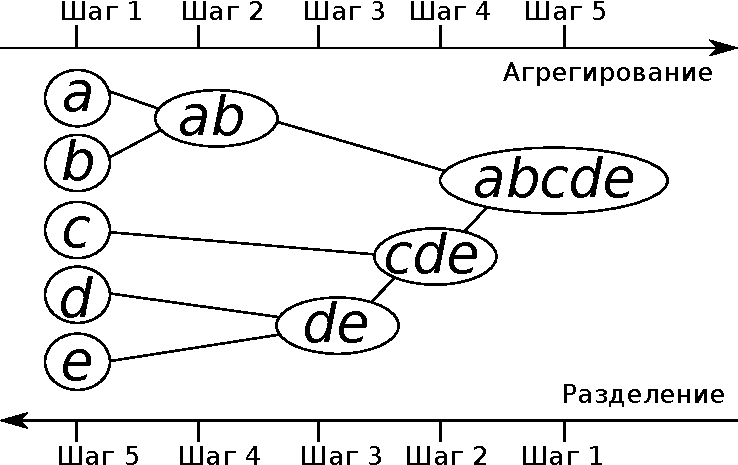
\includegraphics[width=0.5\linewidth]{hclustexp.pdf}
  \caption{Иерархический кластерный анализ}
  \label{fig:hclustdescr}
\end{figure}


% FIXME: адаптировать к процедуре РС
Процесс поиска представляет собой процедуру определения «ближайшего» (наилучшего) кластера, изначально пользователю предлагаются разные варианты недвижимости из разных кластеров, например, квартира, дом или участок. В свою очередь\textbf{ у этих кластеров имеются свои параметры}, такие как «тип строения», кирпичное, деревянное, панельное и другие здания. При выборе такого или иного варианта недвижимости и типа строения, пользователю выводятся предложения о недвижимости с наиболее «близкими» исходными данными основанные на кластеризации.

\begin{figure}[htbp]
  \centering

  \caption{Агломеративный метод кластерного анализа}
  \label{fig:clusagloshow}
\end{figure}

Рассмотрим $Ι = (Ι_1, Ι_2, \ldots Ι_n)$ как множество кластеров $\{Ι_1\}$, $\{Ι_2\}$, $\ldots$ $\{Ι_n\}$. Выберем два из них, например, $Ι_i$ и $Ι_j$, которые в некотором смысле более близки друг к другу и объединим их в один кластер. Новое множество кластеров, состоящее уже из $n-1$ кластеров, будет: $\{Ι_1\}$, $\{Ι_2\}$, $\ldots$, $\{Ι_i , Ι_j\}$, $\ldots$, $\{Ι_n\}$. Повторяя процесс, получим последовательные множества кластеров, состоящие из $(n-2)$, $(n-3)$, $(n–4)$ и т.д. кластеров. В конце процедуры можно получить кластер, состоящий из n объектов и совпадающий с первоначальным множеством $Ι = (Ι_1, Ι_2, \ldots Ι_n)$. В качестве меры расстояния возьмем квадрат евклидовой метрики и вычислим матрицу $D= \{d_{i,j}^2 \}$, где $d_{i,j}^2$ -- квадрат расстояния между $Ι_i$ и $Ι_j$.

\begin{figure}[htbp]
  \centering
  \begin{tabular}{|c||c|c|c|c|c|}
    \hline
          & $I_1$ & $I_2$       & $I_3$       & $\ldots$ & $I_n$        \\
    \hline
    \hline
    $I_1$ & 0     & $d_{1,2}^2$ & $d_{1,3}^2$ & $\ldots$ & $d_{1,n}^2$  \\
    \hline
    $I_2$ &       & 0           & $d_{2,3}^2$ & $\ldots$ & $d_{2,n}^2$  \\
    \hline
    $I_3$ &       &             & 0           & $\ldots$ & $d_{3,n}^2$  \\
    \hline
 $\ldots$ &       &             &             & $\ldots$ & $\ldots$ \\
    \hline
    $I_n$ &       &             &             &          & 0  \\
    \hline
  \end{tabular}
  \caption{Симметричная матрица расстояний}
  \label{fig:disssimm}
\end{figure}
Пусть расстояние между $Ι_i$ и $Ι_j$ будет минимальным: $d_{i,j}^2=\min⁡(d_{i,j}^2,i\neq j)$. Образуем с помощью $Ι_i$ и $Ι_j$ новый кластер $\{Ι_i, Ι_j\}.$

\begin{figure}[htbp]
  \centering
  \begin{tabular}{|c||c|c|c|c|c|c|}
    \hline
                  & $\{I_i,I_j\}$ & $I_1$         & $I_2$         & $I_3$         & $\ldots$ & $I_n$        \\
    \hline
    \hline
    $\{I_i,I_j\}$ &  0            & $d_{i,j,1}^2$ & $d_{i,j,2}^2$ & $d_{i,j,3}^2$ & $\ldots$ & $d_{i,j,n}^2$  \\
    \hline
    $I_1$ & & 0     & $d_{1,2}^2$ & $d_{1,3}^2$ & $\ldots$ & $d_{1,n}^2$  \\
    \hline
    $I_2$ & &      & 0           & $d_{2,3}^2$ & $\ldots$ & $d_{2,n}^2$  \\
    \hline
    $I_3$ & &      &             & 0           & $\ldots$ & $d_{3,n}^2$  \\
    \hline
 $\ldots$ & &      &             &             & $\ldots$ & $\ldots$ \\
    \hline
    $I_n$ & &      &             &             &          & 0  \\
    \hline
  \end{tabular}
  \caption{Новая матрица расстояний}
  \label{fig:disssimmnew}
\end{figure}
Для новой матрицы $(n-2)$ строки взяты из предыдущей, а первая строка вычислена заново. Исходно определено расстояние лишь между одноэлементными кластерами, но надо определять расстояния и между кластерами, содержащими более чем один элемент. Это можно сделать различными способами, в зависимости от выбранного способа мы получаем алгоритмы кластерного анализа с различными свойствами. Можно, например, положить расстояние между кластером $i + j$ и некоторым другим кластером $k$, равным среднему арифметическому из расстояний между кластерами $i$ и $k$ и кластерами $j$ и $k$:
\[d_{i+j,k}=(d_{i,k}+d_{j,k})/2.\]
Но можно также определить его как минимальное из этих двух расстояний:
\[d_{i+j,k}=\min⁡(d_{i,k}+d_{j,k}).\]
Подобная операция выполняется на каждом шаге агломеративного иерархического метода кластерного анализа.

В результате получается древовидная структура, представленная на рисунке~\ref{fig:hclusttree}
\begin{figure}[htbp]
  \centering
  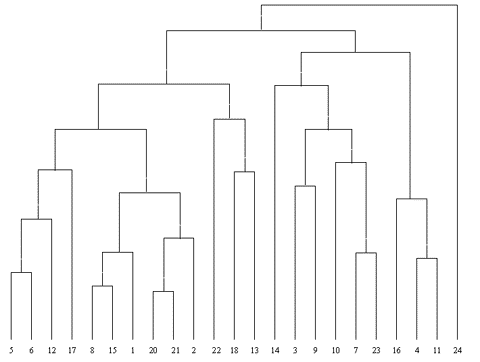
\includegraphics[width=0.5\linewidth]{hclustexample.png}
  \caption{Пример дерева кластерного анализа \protect\cite{aicourse}}
  \label{fig:hclusttree}
\end{figure}
В результате реализован алгоритм кластерного анализа при подборе оптимальных вариантов недвижимости. Существуют методы, которые строят подобные деревья но в обратном направлении, т.е. в отличии от агломеритвного метода они разделяют все множество объектов на подмножества.  Методы второго классу удобны, если множество объектов большое и не требуется строить дерево до листовых вершин. При беглом поиске библиотеки, реализующей метод второго типа, такую библиотеку обнаружить нам, к сожалению, в среде .NET не удалось, поэтому в данной работе использован \emph{агломеративный} метод из библиотеки \textsc{ALGLIB} \cite{alglib}. % Я на втором мониторе открыл результат, чтоб не переключать экраны.

\subsection{Функция меры схожести для объектов недвижимости}

Как было сказано выше применение методов кластерного анализа неразрывно связано с построением матрицы различия между объектами исходного множества. В нашем случае необходимо задать меру схожести между объектами недвижимости. Каждый объект недвижимости задан атрибутами, поэтому необходимо построить функцию сравнения двух объектов как совокупность функции сравнения их атрибутов.

Согласно диаграмме классов, изображенной на рисунке~\ref{fig:classdiagram} (стр.~\pageref{fig:classdiagram}), атрибуты разнородны (описываются различными типами данных), поэтому необходимо задать для каждого типа данных, фактически для каждого атрибута, функцию сравнения $d_k(i,j):A_k\to [0,1]$, где $k$ -- номер атрибута $k=1,2,\ldots,m$, $m$ -- число атрибутов в описании объекта.

\begin{table}[htbp]\footnotesize
  \caption{Перечень функций сравнения атрибутов объекта недвижимости}
  \label{tab:attrdiff}
  \centering
  \begin{tabular}{|l|p{5cm}|c|c|}
    \hline
    Атрибут & Способ вычисления & $v_k, \%$ & Формула \\
    \hline
\texttt{string Name} & не используется & & \\
    \texttt{ILocation Location} & совпадение значений & 10 & $d_k(i,j) = \left\{
                                                          \begin{array}{ll}
                                                            0, & \mbox{если\ \ } a_i=a_j,\\
                                                            1, & \mbox{если\ \ } a_i\neq a_j,
                                                          \end{array}
                                                          \right. (\star)$
    \\
\texttt{string Address} & --''-- & 10 & \\
\texttt{float Price} & относительная разница величины & 25 & $d_k(i,j) = \frac{|a_i^k-a_j^k|}{a_i^k+a_j^k}, a_i^k+a_j^k>0\quad(\star\star)$\\
\texttt{CurrencyEnum CurrencyType} & не используется  & & \\
\texttt{float Area} & относительная разница величины  & 35 & $(\star\star)$\\
\texttt{AreaUnits AreaUnit} & не используется & &\\
\texttt{string ImageURL} & --''-- & & \\
\texttt{string URL} & --''-- & & \\
\texttt{int Rooms}  & относительная разница величины  & 100 & $(\star\star)$\\
\texttt{int RoomsOffered} &  --''--   & 100 & $(\star\star)$\\
\texttt{int Floor}  &  --''--   & 30 & $(\star\star)$\\
\texttt{int FloorTotal}  &  --''--   & 10 & $(\star\star)$\\
\texttt{BuildingEnum BuildingType}  & совпадение значений & 30 & $(\star)$\\
\texttt{IBuild\ldots{} BuildingSeries}  & --''-- & 30 &  $(\star)$\\
\texttt{PropertyEnum PropertyType} & --''-- & 30 &  $(\star)$\\
\texttt{CategoryEnum Category} & --''-- (вид объекта: квартира, дом и т.д.) & 100 &  $(\star)$\\
\texttt{string Description} & не используется & & \\
    \texttt{string GUID} & --''-- & & \\
    \hline
  \end{tabular}

  В таблице $v_k$ -- весовой коэффициент $k$-го атрибута.
\end{table}

Далее значения по всем атрибутам необходимо свести в одно, используем формулу манхеттеновского расстояния:
\[
  d(i,j)=\frac{\sum\limits_{k=1}^m|v_k\cdot d_k(i,j)|}{\sum\limits_{k=1}^m v_k}, \qquad 0\leqslant d_(i,j)\leqslant 1.
\]
где $v_k$ -- весовой коэффициент, который задает степень <<важности>> данного атрибута. В нашем случае использован ряд значений от 0 до 100, где числа до 15 обозначают неважный атрибут, 15-50 -- атрибут <<средней>> важности, и число, большее 50 обозначает важный атрибут. Принятая нами система, таким образом, задает атрибуты типа жилья и <<количество комнат>> самыми важными в сравнении. Меняя соотношение весовых коэффициентов можно строить новые варианты кластеров.

\section{Тестирование системы}
Тестирование программной системы проводилось при помощи двух подходов:
\begin{itemize}
\item разработка функциональных тесто и тестов корректности;
\item тестирование вручную несколькими <<виртуальными>> пользователями;
\end{itemize}

\subsection{Автоматическое функциональное тестирование}
xUnit - это собирательное название семейства фреймворков для модульного тестирования, структура и функциональность которых основана на SUnit, предназначавшегося для языка программирования Smalltalk.

\subsection{Структуризация множества объектов недвижимости}
Перед тем, как начать тестирование функций рекомендательной системы можно выполнить процесс структуризации объектов недвижимости, т.е. разбить все множество объектов на подмножества при помощи иерархического кластерного анализа. Далее экспериментальным путем подбирается количество кластеров для представления структуры рынка недвижимости региона.

Процедура выполняется экспертом при помощи интерфейса пользователя по адресу \url{http://127.0.0.1:8080/analysis}. Пример использования данного режима информационной системы приведен на рисунке~\ref{fig:exclus1}.
\begin{figure}[htbp]
  \centering
  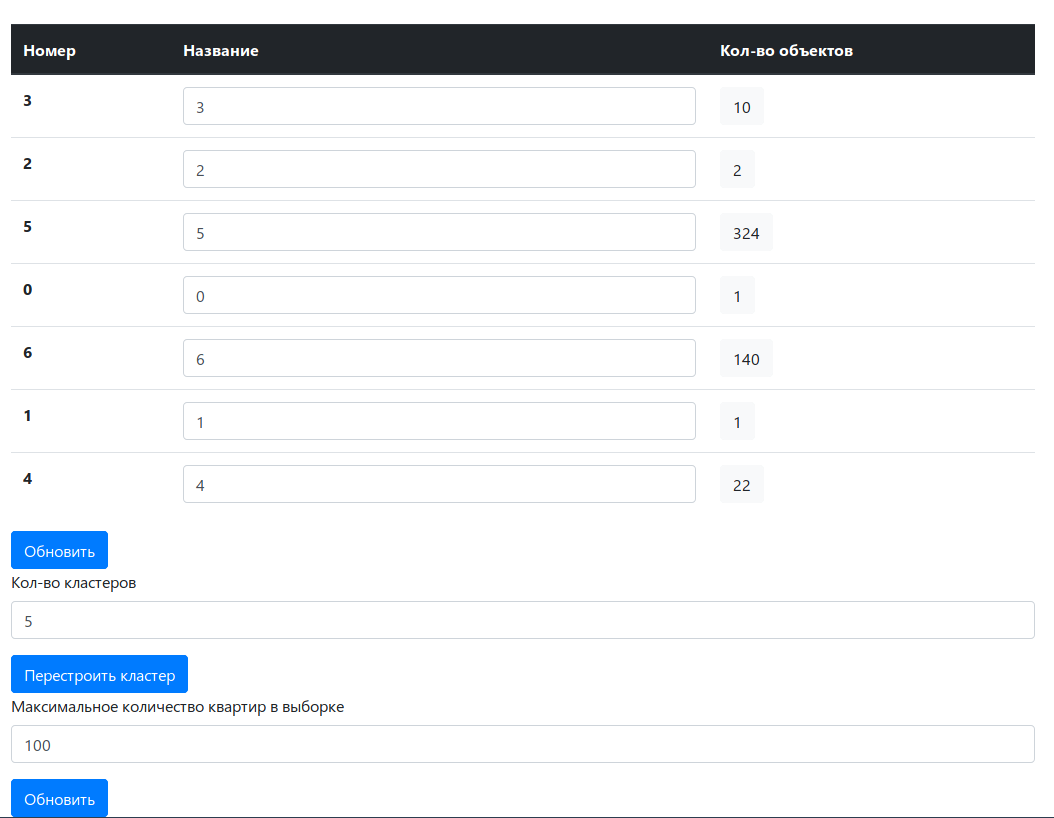
\includegraphics[width=0.8\linewidth]{screen-cluster-start.png}
  \caption{Проведение структуризации данных рынка недвижимости (начальный этап)}
  \label{fig:exclus1}
\end{figure}

Экран представляет собой перечень пронумерованных кластеров (подмножеств), начиная с 0.  Страница позволяет выполнить следующие операции:
\begin{itemize}
\item задать название подмножеству: в поле соответствующего кластера вписывается строка символов (название кластера), например <<Дома>>, нажимается верхняя кнопка <<Обновить>>, при этом все кластеры с одинаковым названиями объединяются в один общий кластер, и процедуры оценивания будут выполнятся только с объектами данного объединения;
\item перестроить построенное дерево анализа, при этом выделив из него задан аза количество кластеров, для этого надо в поле <<Кол-во кластеров>> ввести число требуемых кластеров и нажать кнопку <<Перестроить кластер>>;
\item перезапустить процедуру построения дерева кластерного анализа заново, нажав нижнюю кнопку <<Обновить>>, при этом предварительно можно указать на каком количестве случайно выбранных объектов недвижимости требуется выполнять данную операцию.
\end{itemize}

\subsection{Тестирование системы пользователями}


\begin{thebibliography}{99}
\bibitem{slopeone} Daniel Lemire, Anna Maclachlan. Slope One Predictors for Online Rating-Based Collaborative. [Электронный ресурс] URL:~\url{http://cogprints.org/4031/1/lemiremaclachlan_sdm05.pdf} (дата доступа: 10.05.2018)
\bibitem{alglib} ALGLIB -- C++/C\# numerical analysis library. [Электронный ресурс] URL:~\url{http://www.alglib.net/} (дата доступа: 10.05.2018)
\bibitem{aicourse} Иерархическое группирование\;// Курс лекций по предмету "Основы проектирования систем с искусственным интеллектом". Составитель -- С.~Л.~Сотник. [Электронный ресурс] URL:~\url{http://www.codenet.ru/progr/alg/ai/htm/gl3_11.php} (дата доступа: 10.05.2018)
\bibitem{entityframework} Руководство по Entity Framework [Электронный ресурс] URL:~\url{https://metanit.com/sharp/entityframework/} (дата доступа: 10.05.2018)
\end{thebibliography}

\appendix
\renewcommand{\chaptername}{ПРИЛОЖЕНИЕ}
\renewcommand{\thechapter}{\arabic{chapter}}
\chapter{Листинг основных модулей}

\end{document}

%%% Local Variables:
%%% mode: latex
%%% TeX-master: t
%%% End:
